% This file was automatically generated by flatten.py
% Source: manuscript.tex
% Do not edit this file directly — edit the source files instead.
% ---------------------------------------------------------------

% plos_latex_template.tex
% Version 3.7 Aug 2025 — refactored for shared preamble
%
% SUBMISSION NOTE: PLOS requires a single flat .tex file.
% Before submitting, run: ./rerunpdf.sh -f plos_latex_template
% which calls flatten.py to inline all \input commands.
% -------------------------------------------------------------------------

\documentclass[10pt,letterpaper]{article}

% PLOS layout
\usepackage[top=0.85in,left=2.75in,footskip=0.75in]{geometry}
\usepackage{changepage}
\usepackage{cite}

% -------------------------------------------------------------------------
% SHARED PACKAGES AND MACROS
% -------------------------------------------------------------------------

% --- begin input: preamble_shared ---
% preamble_shared.tex
% Shared packages and macros for plos_latex_template.tex and supplement_main.tex
% DO NOT add layout/geometry/header packages here — those are file-specific.
% -------------------------------------------------------------------------

% Core math
\usepackage{amsmath,amssymb}

% Additional characters
\usepackage{textcomp,marvosym}

\usepackage[final,commentmarkup=footnote]{changes}  % use mode draft to show changes

\definechangesauthor[name={Reviewer 1}, color=blue]{R1}
\definechangesauthor[name={Reviewer 2}, color=orange]{R2}
\definechangesauthor[name={Reviewer 3}, color=teal]{R3}
\definechangesauthor[name={Multiple Reviewers}, color=magenta]{MR}
\definechangesauthor[name={Editor}, color=brown]{ED}
\definechangesauthor[name={PLOS Final Submission}, color=violet]{PLOS}


% Hyperlinks (nameref required for SI cross-references)
\usepackage{nameref,hyperref}

% Color (table shading)
\usepackage[table]{xcolor}

% Table utilities
\usepackage{array}
\usepackage{booktabs}

% Thick rule helpers (used in main manuscript tables)
\newcolumntype{+}{!{\vrule width 2pt}}
\newlength\savedwidth
\newcommand\thickcline[1]{%
  \noalign{\global\savedwidth\arrayrulewidth\global\arrayrulewidth 2pt}%
  \cline{#1}%
  \noalign{\vskip\arrayrulewidth}%
  \noalign{\global\arrayrulewidth\savedwidth}%
}
\newcommand\thickhline{%
  \noalign{\global\savedwidth\arrayrulewidth\global\arrayrulewidth 2pt}%
  \hline
  \noalign{\global\arrayrulewidth\savedwidth}%
}

% -------------------------------------------------------------------------
% SHARED MACROS
% -------------------------------------------------------------------------

% Simulation output symbols
\newcommand{\TAT}[1]{\ensuremath{\mathrm{TAT}_{#1}}}
\newcommand{\VOL}[1]{\ensuremath{\mathrm{Vol}_{#1}}}
\newcommand{\deltaVol}[1]{\ensuremath{\Delta \mathrm{Vol}_{#1}}}
\newcommand{\deltaVolNorm}[1]{\ensuremath{\mathcal{V}_{#1}}}

% Anatomical abbreviations
\newcommand{\LV}{LV}
\newcommand{\RV}{RV}
\newcommand{\LA}{LA}
\newcommand{\RA}{RA}
\newcommand{\SAN}{SAN}
\newcommand{\UKBB}{UKBB}

% Clinical group abbreviations
\newcommand{\Ctl}{$C$}
\newcommand{\HF}{$HF$}
\newcommand{\HFN}{$HF_N$}
\newcommand{\HFW}{$HF_W$}
% --- end input:   preamble_shared ---


% -------------------------------------------------------------------------
% PLOS-SPECIFIC LAYOUT (not shared with supplement)
% -------------------------------------------------------------------------

% Line numbers
\usepackage[right]{lineno}

% Ligatures
\usepackage[nopatch=eqnum]{microtype}
\DisableLigatures[f]{encoding = *, family = * }

% Captions
\usepackage[aboveskip=1pt,labelfont=bf,labelsep=period,justification=raggedright,singlelinecheck=off]{caption}
\renewcommand{\figurename}{Fig}

% Bibliography style
\bibliographystyle{plos2025}
\makeatletter
\renewcommand{\@biblabel}[1]{\quad#1.}
\makeatother

% Header/footer
\usepackage{lastpage,fancyhdr,graphicx}
\usepackage{epstopdf}
\pagestyle{fancy}
\fancyhf{}
\rfoot{\thepage/\pageref{LastPage}}
\renewcommand{\headrulewidth}{0pt}
\renewcommand{\footrule}{\hrule height 2pt \vspace{2mm}}
\fancyheadoffset[L]{2.25in}
\fancyfootoffset[L]{2.25in}
\lfoot{\today}

% Text layout
\raggedright
\setlength{\parindent}{0.5cm}
\textwidth 5.25in
\textheight 8.75in

% -------------------------------------------------------------------------
% CROSS-DOCUMENT REFERENCES (supplement ↔ manuscript)
% -------------------------------------------------------------------------
\usepackage{xr}
\externaldocument{supplement_main}

% -------------------------------------------------------------------------
% MANUSCRIPT-SPECIFIC MACROS (not needed in supplement)
% -------------------------------------------------------------------------
\newcommand{\autor}{%
    Jos\'e Alonso Sol\'is-Lemus\textsuperscript{1,\Cross,*},
    Rosie K. Barrows\textsuperscript{1,\Cross},
    Cristobal Rodero\textsuperscript{1},
    Marina Strocchi\textsuperscript{1,6},
    Natalie Montarello\textsuperscript{2},
    Nishant Lahoti\textsuperscript{2},
    Cesare Corrado\textsuperscript{1},
    Abdul Qayyum\textsuperscript{1},
    Shahrokh Rahmani\textsuperscript{1},
    Caroline Roney\textsuperscript{3},
    Gernot Plank\textsuperscript{4,5},
    \replaced[id=PLOS, comment={EM: correct spelling per author}]{Christoph}{Cristoph} Augustin\textsuperscript{4,5},
    Hao Xu\textsuperscript{2},
    Alistair Young\textsuperscript{2},
    Pras Pathmanathan\textsuperscript{7},
    Ronak Rajani\textsuperscript{2},
    Steven A. Niederer\textsuperscript{1,8}%
}

\newcommand{\titulo}{%
    Assessing the Importance of Sex and Disease-Specific Anatomy in
    Electrophysiology and Mechanical Simulations with a Newly Developed
    Public Virtual Cohort of Four-Chamber Heart Models%
}

% =========================================================================
\begin{document}
\vspace*{0.2in}

\begin{flushleft}
{\Large\textbf{\titulo}}
\newline
\\
\autor
\\
\bigskip
\textbf{1} National Heart and Lung Institute, Imperial College London, UK \\
\textbf{2} School of Biomedical Engineering and Imaging Sciences, King's College London, UK \\
\textbf{3} Queen Mary University of London, UK \\
\textbf{4} Gottfried Schatz Research Center, Division of Medical Physics and Biophysics, Medical University of Graz, Austria \\
\textbf{5} BioTechMed-Graz, Austria \\
\textbf{6} Cardiac Rhythm Management, Medtronic, London, UK \\
\textbf{7} Food and Drug Administration, United States \\
\textbf{8} Alan Turing Institute, London, UK \\
\bigskip

\Cross These authors share first authorship.

* j.solis-lemus@imperial.ac.uk
\end{flushleft}

\section*{Abstract}
    This work presents a study on how differences in cardiac
    anatomy attributed to sex and disease can influence cardiac
    electrophysiology and mechanics using a virtual cohort of four-chamber
    heart models.
    Patient anatomy varies across sex and disease.
    However, capturing this variation in in-silico studies remains poorly accounted for,
    with studies often using either single representative cases or imbalanced virtual cohorts.
    Whole-heart electromechanics models incorporate the patient's anatomy,
    electrophysiology and mechanics across different scales, from molecular,
    tissue and whole-heart and circulatory system levels.
    However, cardiac models are typically built from one or a small number of anatomies,
    with sex rarely reported and the effects of anatomical variability, which include those due to
    sex or disease, largely unexplored.
    This limits clinical translation and reduces regulatory credibility.

    We developed fifty patient-specific anatomical models of 25 male and 25 female hearts in
    heart failure and control cases.
    We ran benchmark passive inflation and paced activation simulations with consistent parameters and
    boundary conditions across cases to isolate the impact of anatomical variations with sex and disease.

    Heart failure models exhibited increased chamber volumes, larger volume changes during inflation,
    and delayed activation times relative to controls.
    These trends were consistent across sexes, although right ventricular activation showed a significant
    sex-based difference.

    Variations in anatomy with sex and disease have a significant impact on cardiac simulations,
    which support the inclusion of multiple heart anatomical models in in-silico trials.
    The resulting virtual cohort captures key anatomical variability and is publicly available at
    \url{https://doi.org/10.5281/zenodo.19351401} and our code is available
    at \url{https://github.com/OpenHeartDevelopers/cemrg-heartbuilder}.

\section*{Author summary}
Understanding how sex and disease affect the heart's electrical and mechanical behaviour is essential
for developing accurate and credible computational models.
In this study, we built a balanced virtual cohort of fifty patient-specific, four-chamber heart models
from male and female individuals with and without heart failure.
We designed a single, streamlined pipeline to generate these models and ran benchmark simulations of
electrical activation and passive inflation to evaluate how anatomical differences influence cardiac function.

We found that heart failure models showed larger chamber volumes, greater volume changes, and
delayed activation times compared with controls.
These patterns were consistent between sexes, although right ventricular activation showed a clear
sex-related difference. Our results demonstrate that anatomical variability across sex and disease
has a measurable effect on cardiac simulations.
By releasing this virtual cohort and its underlying pipeline publicly, we aim to support reproducible and
transparent in-silico studies and to advance the use of virtual populations in regulatory and clinical
applications.

\linenumbers


% --- begin input: sections/intro_bis ---
\section{Introduction}
Patient-specific computational models and simulations of the heart have increasingly  
been used to develop and guide clinical therapies~\cite{solis-lemus2023_reproducibility},
supporting the  
design~\cite{gray-2018-models_design,vanderlaan-2024-models_design}, 
evaluation~\cite{niederer-2019-models_evaluation,sung-2024-models_evaluation}, 
and delivery~\cite{lee-2018-models_delivery,dokuchaev-2023-models_delivery}
of innovative clinical therapies.
These models could advance personalised medicine by enabling the development and 
in-silico testing of therapies tailored to the anatomical and physiological features of individual patients.
However, the creation of credible and trustworthy cardiac models remains 
challenging~\cite{pras2018-intro-regulatory,jaffery-2024-review}.

There is growing support for the use of simulations for regulatory submission by the 
Medicines and Healthcare products Regulatory Agency~\cite{shepard-2015-mhra}, 
European Medicines Agency~\cite{ema2025_web}, and 
U.S. Food and Drug Administration (FDA)~\cite{jaffery-2024-review,fda2023_web}.
In particular, the FDA has identified scientific gaps and challenges that have limited 
the credibility of simulation models intended for medical use, including
(i) insufficient analytic methods, 
(ii) lack of established credibility assessment tools, 
(iii) absence of best-practice guidelines, and 
(iv) limited availability of high-quality, comprehensive data sets~\cite{fda2023_web}.

Data scarcity remains a fundamental obstacle to the development of robust cardiac models,
particularly the lack of high-quality, sex-balanced, disease-specific patient data. 
Several studies have attempted to bridge this gap through the creation of virtual cohorts that can 
be used for in-silico trials~\cite{strocchi2020_cohort,rodero2021_linking}.
Despite these advances, addressing sex balance in cardiac modeling databases is a persisting challenge. 

The cohort presented by Strocchi et al.~\cite{strocchi2020_cohort} has one 
female patient, while the one presented by Rodero et al.~\cite{rodero2021_linking} 
has 6 out of 20. Finally, in the study by Roney et al.~\cite{Roney2022-predicting} 
on predicting atrial fibrillation recurrence, 28 of the 99 patients were female.
Large virtual heart cohorts have begun to emerge, enabling in-silico trials and population-level 
analyses~\cite{passini2021_virtual,rodero-2021-virtualcohort1000,rodero-2021-virtualcohortextreme}. 
For example, the Strocchi et al.~\cite{strocchi2020_cohort} database has been 
widely used for studies on valve mechanics~\cite{feng2024_db_user}, 
fibrosis detection~\cite{okenov2024_db_user}, and 
arrhythmia modeling~\cite{kaboudian2023_db_user}.

While these cohorts represent valuable tools for the cardiac modelling community, 
they also highlight the challenge of having balanced representation of sex or disease subtypes, and 
workflows for generating new whole-heart cohorts remain poorly defined.

Sex bias is a complex, multi-factorial problem that affects the availability and generalisability 
of data used for computational models and simulations~\cite{steuernagel2023_sex_bias}.
Simulation studies can take considerable time and computational resources, 
which makes it especially relevant to consider whether anatomical differences associated with sex 
or disease influence the results.
The impact of such variation on simulation outcomes as well as on cardiac function is not frequently explored
or understood.
Understanding this relationship is key to determining when sex-specific anatomical data should be 
included in model development and evaluation.

Testing the importance of anatomical variability requires creating sex balanced virtual cohorts. 
However, building a model of the whole heart is a labour-intensive and technically demanding task.
Available solutions involve multiple stages: 
image segmentation, mesh generation, and the assignment of fibre orientations. 
Some approaches have explored the use of deep learning to automate aspects of 
mesh generation~\cite{pak2024_ai_meshes}. 
However, these methods are typically limited to single cardiac chambers rather than 
full four-chamber models.

CemrgApp~\cite{Razeghi2020-cemrgapp} is an open-source medical imaging platform with 
image processing toolkits for cardiovascular research, that has a low barrier to entry 
and low learning curve, putting reproducibility and best practices at the forefront.
CemrgApp has enabled semi-automated creation of high-quality left atrial models and 
has been employed in studies involving 
atrial fibrosis characterisation~\cite{Sim2019-reproducibility}, 
motion quantification~\cite{sillett2024_motion}, and 
regional strain analysis~\cite{sillett2023_strain1}. 
However, the extension of such tools to comprehensive whole-heart modelling, including 
all four chambers, has not been systematically demonstrated or standardised.

In this study, we developed CEMRG Heartbuilder, a Python-based library designed to systematically 
generate patient-specific, four-chamber heart models from clinical computerised tomography (CT) data. 
We applied the workflow to a new cohort of 50 patients (balanced by sex), 
classified into three clinical groups: controls ($n=26$), heart failure with narrow QRS ($n=12$), 
and heart failure with wide QRS ($n=12$). For each case, models were created from a CT scan 
to a simulation-ready mesh with fibres, and subsequently used to run benchmark electrophysiological and 
mechanical simulations. 
The simulations demonstrated the feasibility and robustness of the approach,
and, through the use of uniform material properties, isolated the impact of disease and sex differences 
in anatomy on reference mechanical and electro physiological simulations.

\replaced[id=PLOS, comment={PLOS: Fig (no period)}]{Fig}{Figure}~\ref{fig:heartbuilder_pipeline} 
provides an overview of the pipeline and the resulting cohort.

\begin{figure}[hbpt]
    \centering
    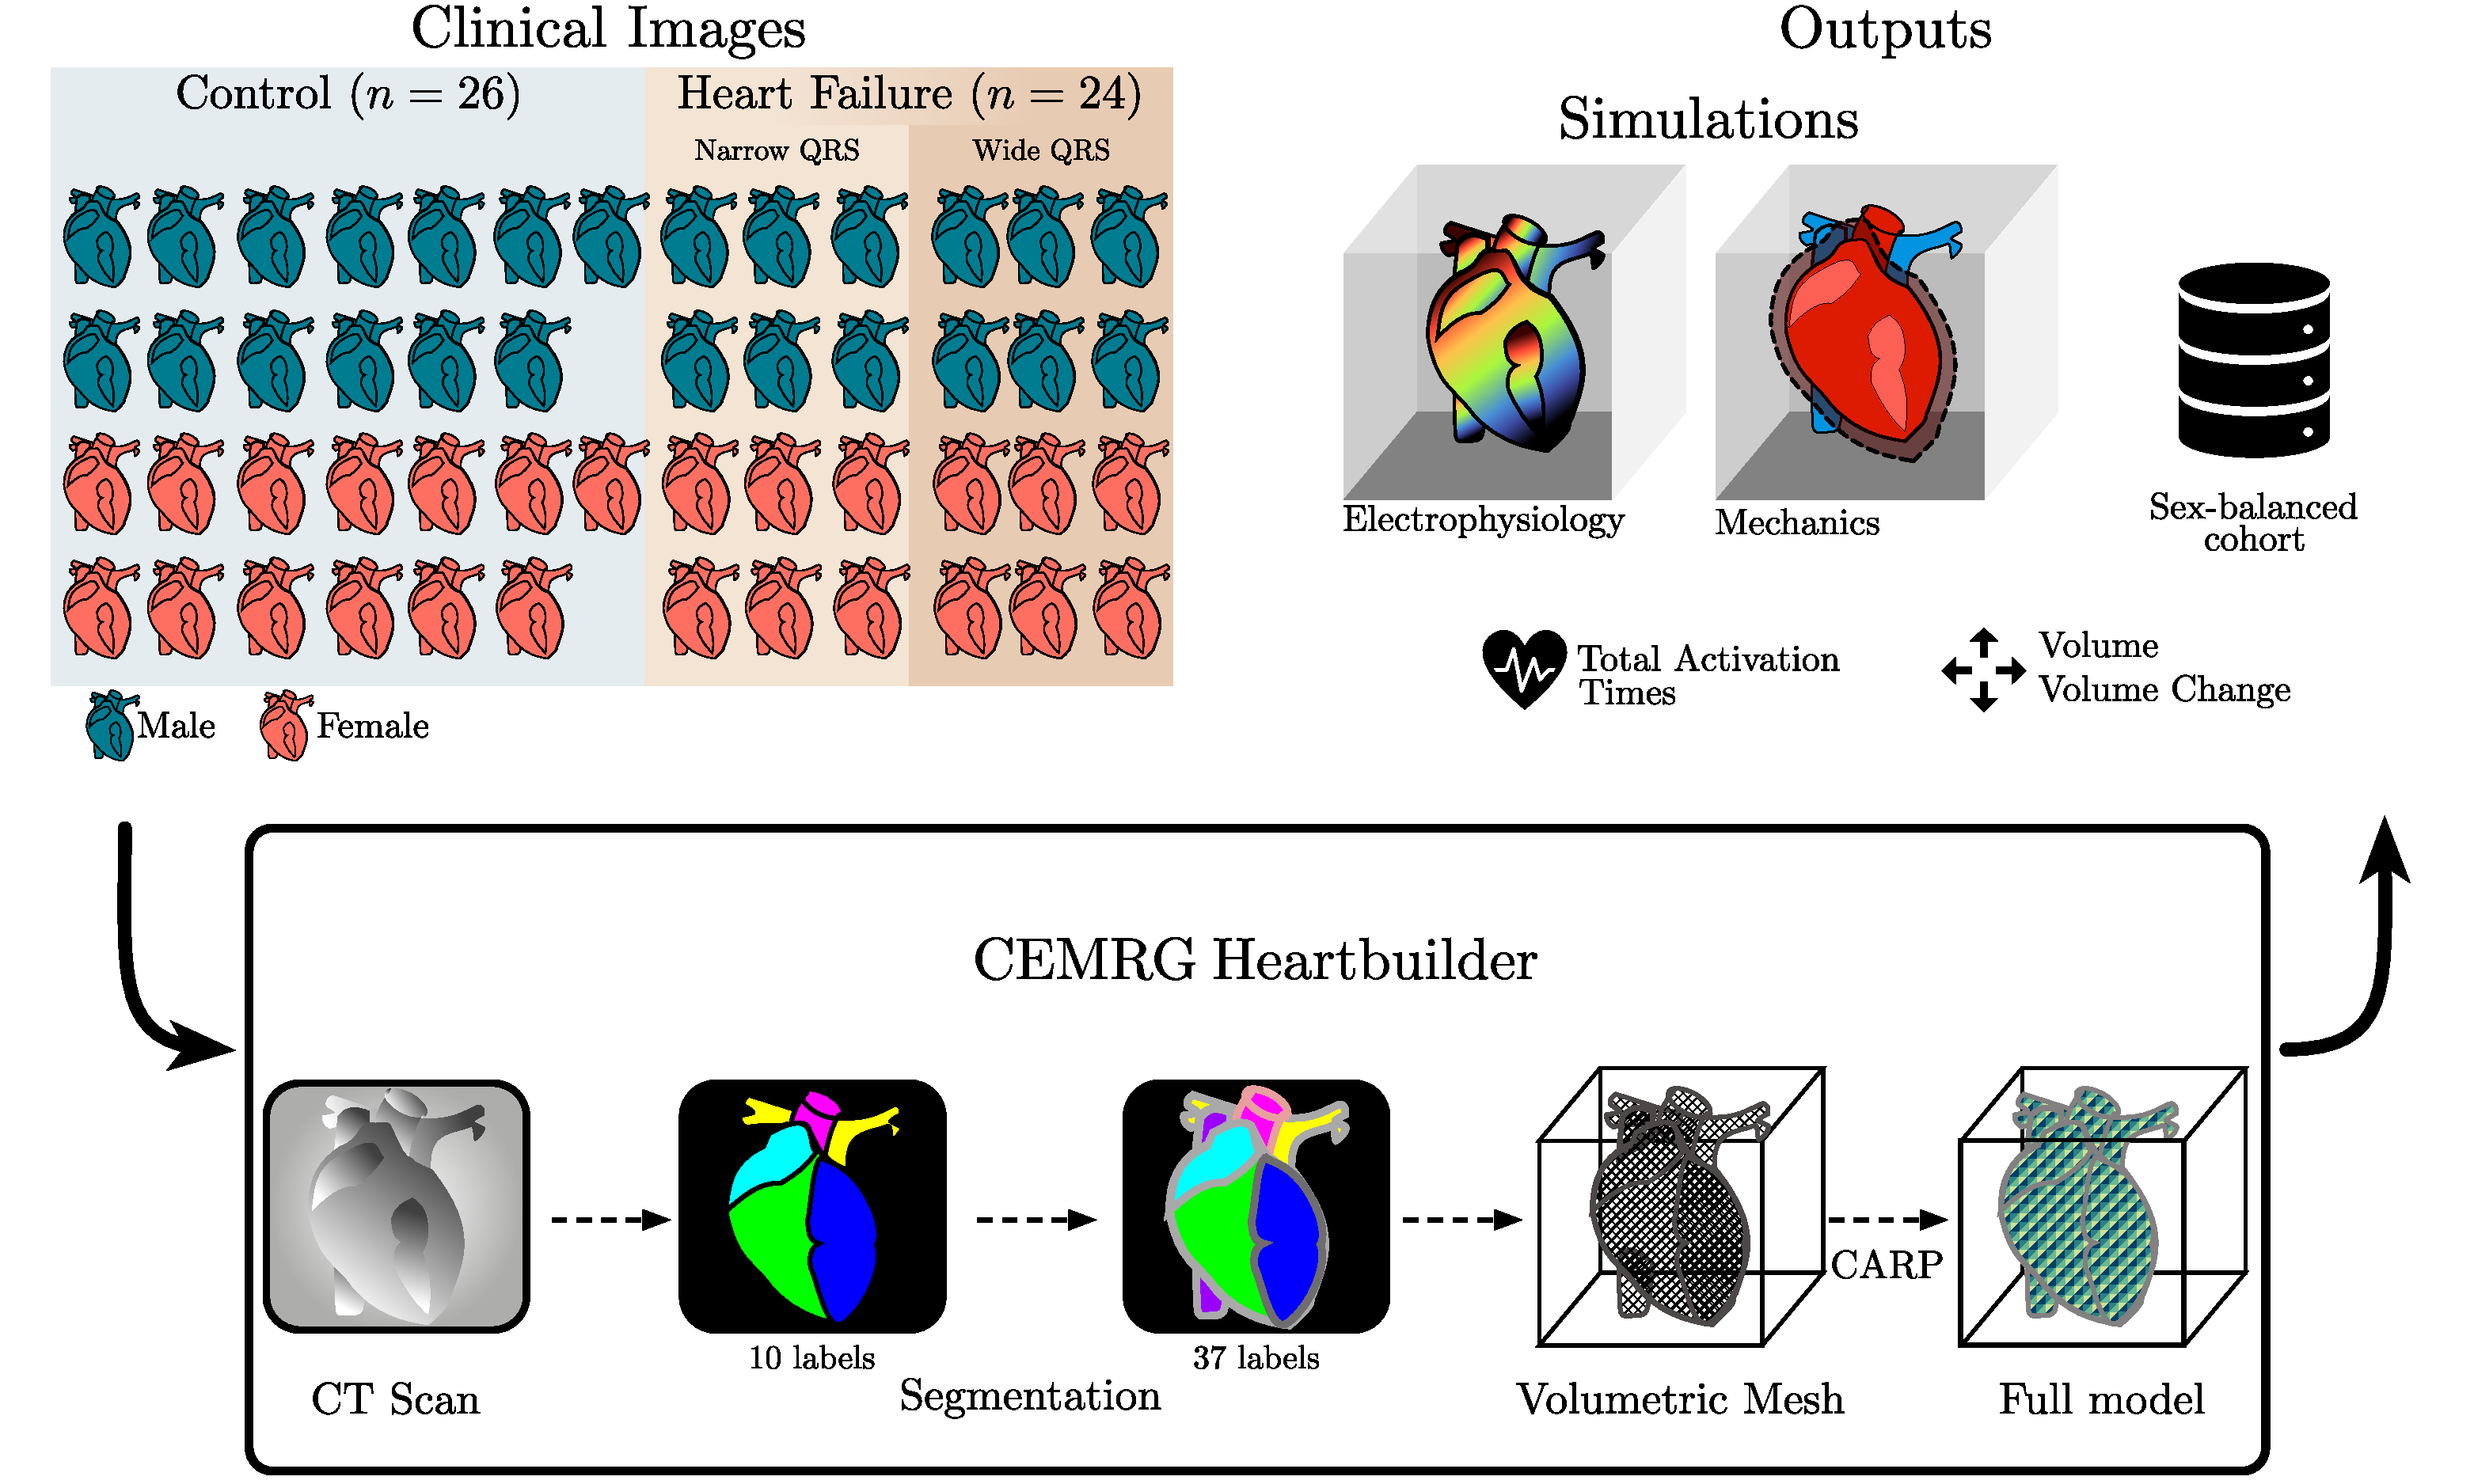
\includegraphics[width=\textwidth]{Fig1}
    \caption[Cohort creation and pipeline overview.]{
        \textbf{Cohort creation and pipeline overview. }
        Starting from clinical CT scans, the workflow performs multi-label segmentation and mesh generation 
        to create simulation-ready models with assigned fibre orientations. 
        A new dataset of 50 patients (26 controls, 24 with heart failure subtypes: narrow QRS and wide QRS) 
        balanced by sex is processed. 
        Resulting models are used in simulations of cardiac electrophysiology and mechanics to extract 
        clinically relevant measurements.
    }
    \label{fig:heartbuilder_pipeline}
\end{figure}


% Thus, the objective is to create and a new cohort of 50 patient-specific, whole-heart models, 
% which include balanced representation of sex and classification into three clinical groups: 
% healthy controls, heart failure with narrow QRS, and heart failure with wide QRS.
% To generate these models in a reproducible and systematic way, we developed the CEMRG Heartbuilder pipeline, 
% a Python-based tool integrating custom image analysis routines with existing platforms
% to produce high-quality, simulation-ready meshes.

% --- end input:   sections/intro_bis ---


% --- begin input: sections/materials ---
\section{Study population}
Fifty cases were processed, creating patient-specific four-chamber heart models. 
The cohort was split into three groups: Controls (\Ctl, $n=26$), Heart Failure (\HF) with narrow QRS (\HFN, $n=12$), 
and HF with wide QRS (\HFW, $n=12$); each group is balanced by sex (50\% Female).
A QRS duration of less than 120 ms is considered narrow. 
Each case consisted of a CT scan, acquired using a consistent imaging 
protocol. The reconstructed meshes represent the cardiac anatomy in a 
static reference configuration. Subsequent mechanical simulations apply 
prescribed endocardial pressures from this baseline geometric state, 
enabling comparison of anatomical effects across the cohort.

\deleted[id=PLOS, comment={PLOS: ethics text relocated to Methods/Ethics Statement}]{
    The study was conducted under ethical approval titled
    Retrospective analysis of cardiac imaging datasets for development of novel biomarkers study
    (Short title: RAIDER),
    approved by GSTT,
    reference number 306914,
    protocol version 1.0 01/10/2021.
}
A summary of the cohort's demographics is presented in Table~\ref{tab:materials-demographics}. 
Summary statistics include the number of participants per group, age, 
ejection fraction (EF) as a percentage, and QRS duration in milliseconds (ms). 
Male control cases were patients with no known cardiac disease or symptoms. 
Five cases had no echocardiography data available and 1 case had no ECG.
% echocardiography was therefore not performed in these patients who largely 
% originated from the rapid access chest pain clinic. 

\begin{table}[hbpt]
    \centering
    \caption[Summary of the 50-patient cohort demographics]{
        \textbf{Summary of the 50-patient cohort demographics, grouped by sex and condition. }
        See text for full description of the cohort and the conditions.
        Abbreviations: M=Male, F=Female, HF=Heart Failure, \HFN=HF with Narrow QRS duration, 
        \HFW=HF with Wide QRS duration.
    }
    \vspace{1em} 
    \begin{tabular}{c|cccc}
                   & Total  & Age            &  EF (\%)        & QRS duration (ms)\\
        \hline
        \hline 
        $M_C$      & 13 & $53.4\pm 12$   &  $58.7\pm 4 (n=8)$ & $90.3\pm 8, (n=12)$\\
        $M_{HF_N}$ &  6 & $53.8\pm 13.8$ & $34.4\pm 14.2$ & $103\pm 7.8$     \\
        $M_{HF_W}$ &  6 & $67.3\pm 16 $  & $38.5\pm 8$    & $163.8\pm 18 $   \\
        \hline 
        $F_C$      & 13 & $49.5\pm 9.8$  & $58.8\pm 4.3$  & $87\pm 1 2.76 $  \\
        $F_{HF_N}$ &  6 & $61\pm 11.4$   & $43.6\pm 7.1$  & $88.3\pm 9.6 $   \\
        $F_{HF_W}$ &  6 & $59.2\pm 7 $   & $36.1\pm7.8$   & $144.7\pm 13.3 $ \\
        \hline 
    \end{tabular}
    \label{tab:materials-demographics}
\end{table}
% --- end input:   sections/materials ---


% --- begin input: sections/methods ---

\section{Methods}
\paragraph{Ethics Statement}
\added[id=PLOS, comment={PLOS: Ethics Statement subsection moved here from Study Population per journal style}]{
    The study was conducted under ethical approval titled
    Retrospective analysis of cardiac imaging datasets for development of novel biomarkers study
    (Short title: RAIDER),
    approved by GSTT,
    reference number 306914,
    protocol version 1.0 01/10/2021.
}

We developed CEMRG Heartbuilder, a pipeline for the streamlined creation of simulation-ready meshes, 
generated from a CT scan. 
The pipeline to process the CT scans is based on the work by~\cite{strocchi2020_cohort} 
but streamlined into a single integrated workflow.
Processing of the information consisted of three stages: 
image to mesh analysis, consisting of a multi-stage segmentation (Section~\ref{sec:segmentation}), 
upsampling, and mesh generation (Section~\ref{sec:meshing}); 
mesh processing and model creation, which includes the assignment of fibre orientations
in the ventricles and atria, 
and the tagging of the mesh with the different labels needed for the simulations (Section~\ref{sec:model-creation}); 
and simulations. 
The multi-stage segmentation and mesh extraction substages are open source, 
whilst some of the mesh post-processing and simulation stages use the 
cardiac arrhythmia research package (CARP)~\cite{carp-2003}. 
Note that the modular structure of the CEMRG Heartbuilder allows for third-party projects to be 
included to be made completely open source.

\subsection{Image to Mesh Stage}
\subsubsection{Multi-stage Segmentation}\label{sec:segmentation}
The image to mesh stage consists of a segmentation of the CT scan via the 
deep learning model by~\cite{hao2021_ccta}, 
\replaced[id=PLOS, comment={PLOS: Fig (no period)}]{Fig}{Figure}~\ref{fig:methods-segmentation}a, 
which identifies 10 distinct regions: 
left ventricle myocardium, and blood pools of the left and right ventricles, the left and right atrium, 
the pulmonary artery, the aorta, 
the left and right atrial pulmonary veins, and left atrial appendage. 
Regions are marked in the segmentation with different integer values,
we refer to these as ``labels'' throughout the manuscript.
% The segmentation is a multi-stage process involving training different U-Nets 
% and refining the output of each to produce the final image-to-label 3D U-Net 
% (Figure~\ref{fig:methods-segmentation}a). 
The user then identifies the different labels in the U-Net output, which splits the pulmonary veins 
into the superior and inferior veins. 
The user selects two sets of 3~points to identify the location and orientation of 
the superior and the inferior venae cavae.
A post-processing stage follows, increasing the number of labels to 37 
(\replaced[id=PLOS, comment={PLOS: Fig (no period)}]{Fig}{Figure}~\ref{fig:methods-segmentation}b). 
This stage creates the myocardia, valve planes, and vein rings. 
The myocardia of the right ventricle (\RV), the atria, the aorta and pulmonary artery are extracted
through the use of distance maps, with a user-selected thickness of 3.5mm for the \RV, and 
2mm for the remaining structures and coupling the different regions to ensure no overlap occurs.
A table of the labels is provided in 
\replaced[id=PLOS, comment={PLOS: S3 Table form}]{\ref{tab:s3-labels} Table}{Supplementary Table~\ref{tab:s3-labels}}.
% See the Supplementary material for a detailed explanation of these points' locations and 
% of the evolution of the segmentation as the post-processing stage occurs.

\begin{figure}[hbpt]
    \centering
    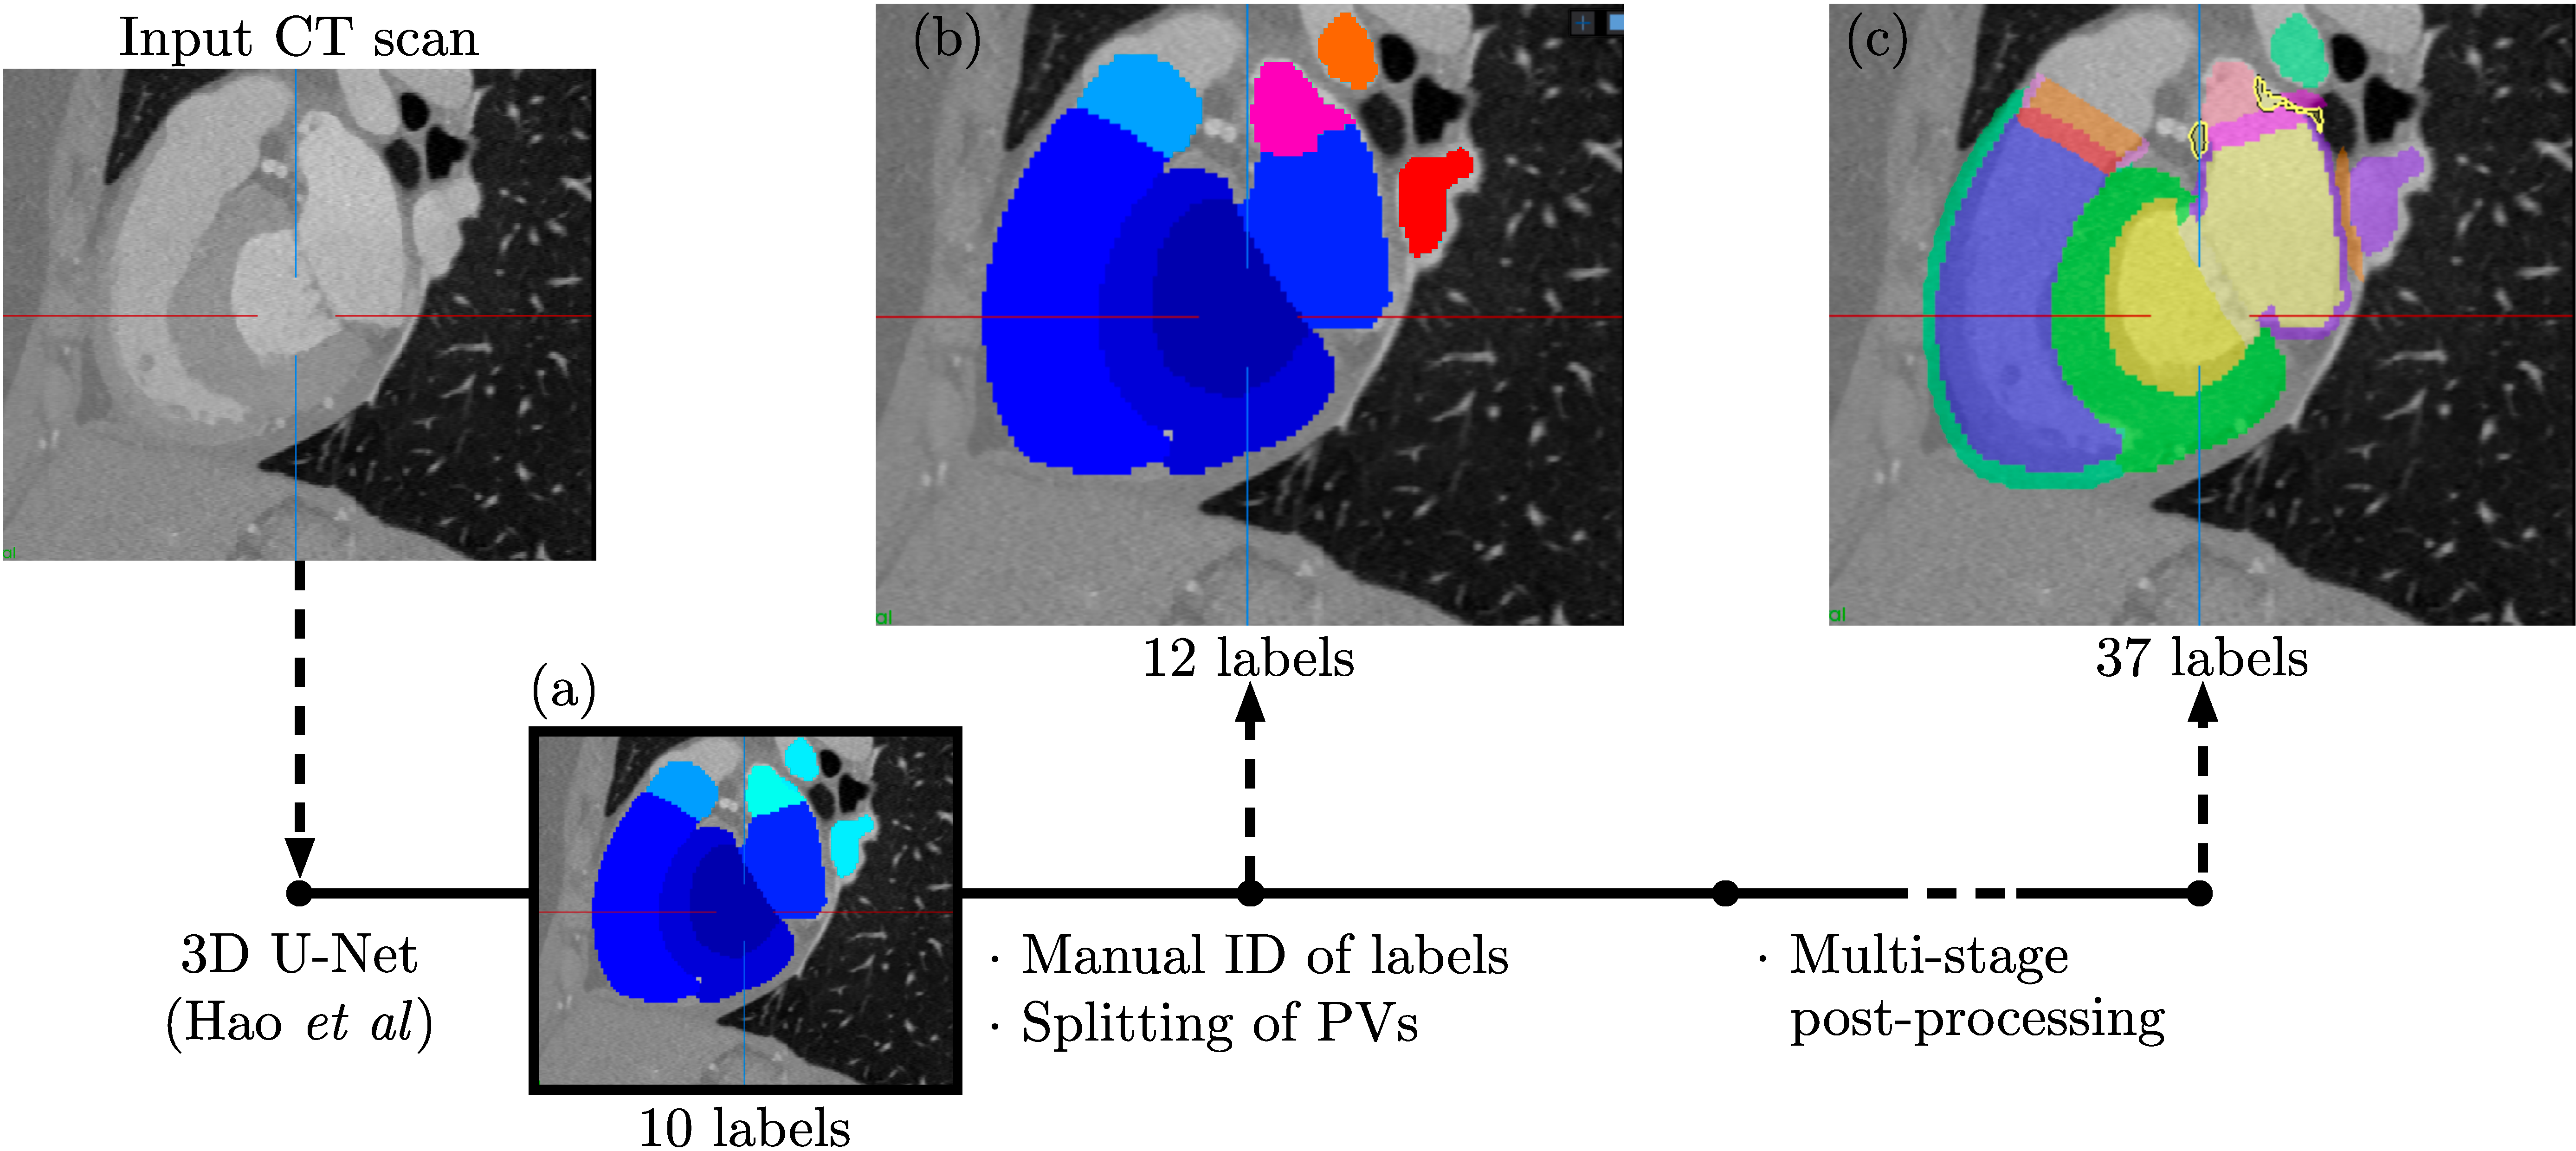
\includegraphics[width=\textwidth]{Fig2}
    \caption[Multi-stage segmentation process. ]{
        \textbf{Multi-stage segmentation process. }
        CemrgApp uses the deep learning model developed by \cite{hao2021_ccta} to segment the heart. 
        (a) The output of the U-Net model, which identifies 10 regions, or ``labels'', 
        as described in the text.
        (b) The output of the intermediate stage, where the user manually 
        splits the pulmonary veins into superior and inferior (marked by contrasting colours).
        (c) The final output of the post-processing stage, where the myocardium of the different structures
        is extracted, increasing the number of labels to 37.
        The final segmented images are then upsampled to an isotropic resolution of 0.1mm and 
        smoothed.
    }
    \label{fig:methods-segmentation}
\end{figure}

CemrgApp aggregates the different workflows through a combination of code running natively on the app and 
a docker wrapper, which calls the segmentation and different post-processing stages. 
The image analysis stage finalises by upsampling the 37-label segmentation to an isotropic resolution of 0.15mm, 
and a applies a smoothing algorithm~\cite{crozier2016_segsmooth}. 

\subsubsection{Conversion to Mesh}\label{sec:meshing}
A volumetric mesh is extracted from the smooth segmentation using a meshing tool developed in-house, 
which comes packaged with CemrgApp and is based on the Computational Geometry Algorithm Library (CGAL)~\cite{cgal}. 
The CGAL mesher generates unstructured volumetric meshes 
composed of linear tetrahedral elements (4 nodes per element). Target 
element edge length was set to approximately 0.5~mm via the 
\texttt{cell\_size} and \texttt{facet\_size} parameters. 
Mesh density is controlled via CGAL parameters 
(\texttt{facet\_size}, \texttt{cell\_size}, \texttt{facet\_distance}), 
which are specified globally for the entire heart geometry. Complete
parameter specifications are provided in \replaced[id=PLOS, comment={PLOS: S2 Table form}]{\ref{tab:s2-cgal-params} Table}{Supplementary Table~\ref{tab:s2-cgal-params}}.

The next step is to extract the myocardia, simplify the mesh topology, and relabel the tags using 
meshtool~\cite{Neic2020-meshtool}.
The simplification consists in identifying elements insufficiently connected to neighbours of the same class.
% The element tags of the entire volumetric mesh are cleaned up and relabelled 
% with meshtool~\cite{Neic2020-meshtool}, before removing the blood pools.
A complete description of the CGAL parameters, which can be modified by the user,
is available in 
\replaced[id=PLOS, comment={PLOS: S2 Table form}]{\ref{tab:s2-cgal-params} Table}{Supplementary Table~\ref{tab:s2-cgal-params}}. 
\replaced[id=PLOS, comment={PLOS: Fig (no period)}]{Fig}{Figure}~\ref{fig:methods-mesh} 
shows the output of the meshing process from the smooth segmentation 
to the working mesh re-labelled and with the blood pools removed.
The final simulation-ready models contained a mean of $2.6 \times 10^6$ elements per heart 
(range $1.9$--$4.5 \times 10^6$).

\begin{figure}[hbpt]
    \centering
    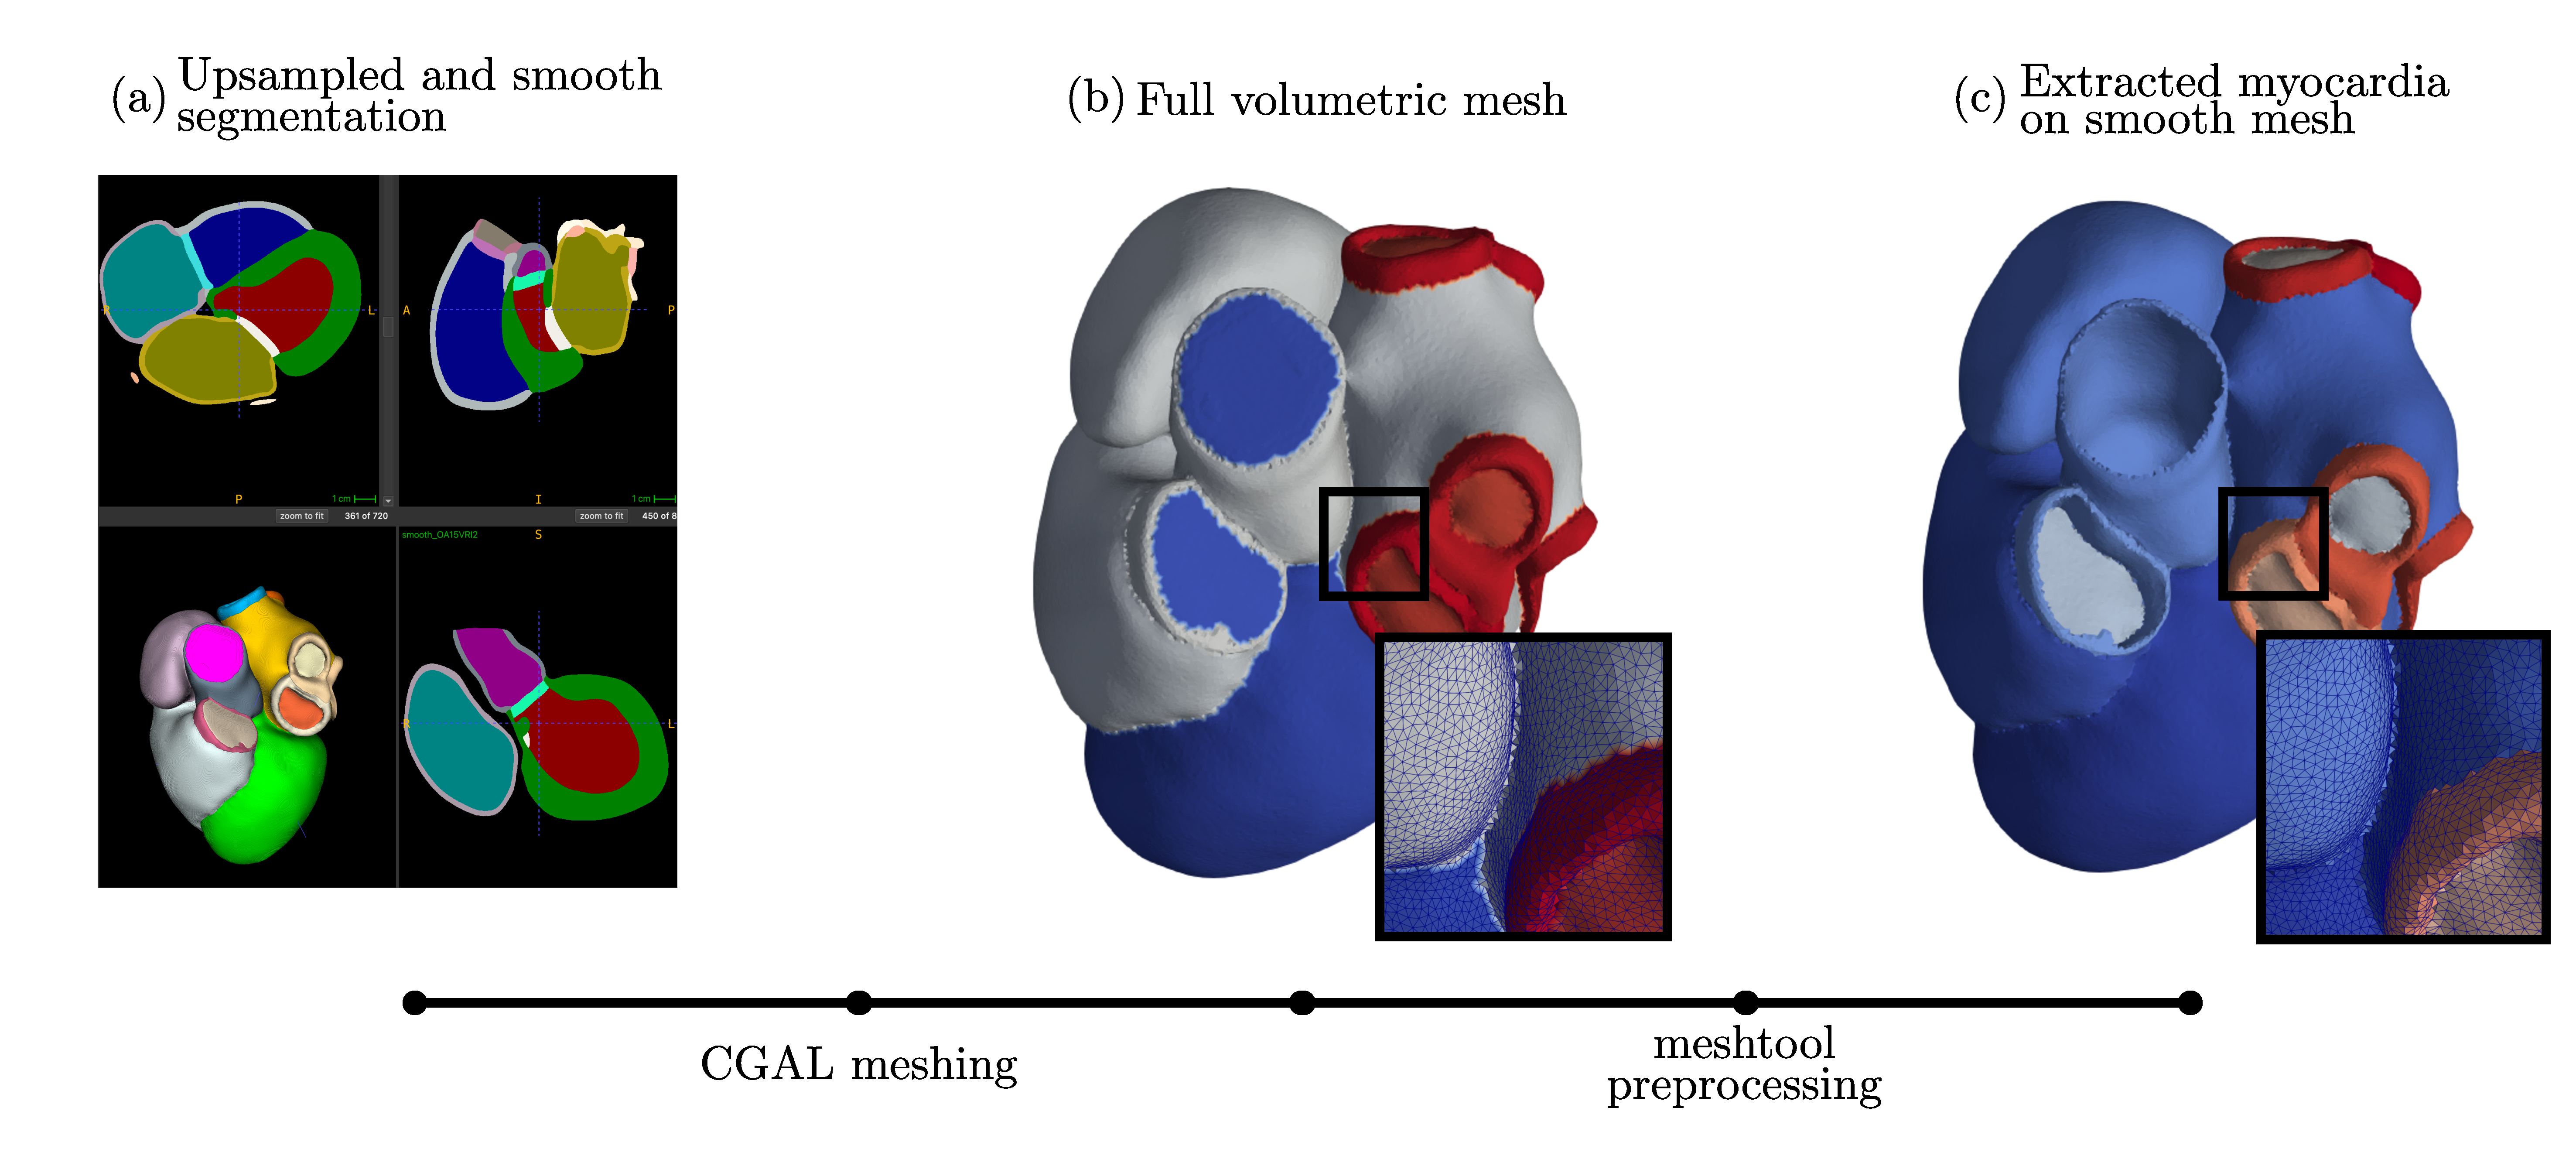
\includegraphics[width=\textwidth]{Fig3}
    \caption[Output of the meshing process.]{
        \textbf{Output of the meshing process from the smooth segmentation to the final working mesh.}
        (a) The upsampled and smooth segmentation. 
        (b) The mesh extracted from the segmentation using the CGAL meshing tool. 
        It contains all the blood pool and myocardium of the different structures.
        (c) The final mesh after the relabelling, cleaning, smoothing, and 
        extracting only the myocardia and valve planes. 
        Other outputs are created from this final process, such as specific endocardial and 
        epicardial surface meshes for the atria, which will be used later in the process.
    }
    \label{fig:methods-mesh}
\end{figure}

\subsection{Mesh Processing and Model Creation}\label{sec:model-creation}
The last stage of the pipeline included takes the smooth mesh and produces 
a model with fibre orientations, tagged with the different labels needed for the simulations.
This stage is run using CARP and meshtool~\cite{Neic2020-meshtool,carp-2003} along with 
the CEMRG Heartbuilder python library. 
\replaced[id=PLOS, comment={PLOS: Fig (no period)}]{Fig}{Figure}~\ref{fig:methods-model-creation} 
shows a visual overview of the model creation stage, 
which is described in detail below.

% Description of UVCs and ventricular fibres:
Universal Ventricular Coordinates (UVCs) are a system of coordinates that 
describe the geometry of the ventricles~\cite{bayer-2018-uvc}.
Additionally to the ventricles, UVCs are also calculated for the atria, 
to provide a system of coordinates defined on the volumetric mesh that facilitated 
the assignment of different tags within the mesh, and of boundary conditions for the 
pericardium.
To achieve this, 
the left and the right atria were treated as an upside down single ventricle,
following the approach described by Strocchi et al.~\cite{strocchi2020_simulating}, 
with the apex manually placed between the two right pulmonary veins and behind the 
supervior vena cava, respectively. 

Atrial fibres are then assigned to the mesh by projecting a rule-based fibre 
field~\cite{labarthe2016_model}
onto the mesh using Universal Atrial Coordinates (UACs)~\cite{Roney2021-atlas}.
Ventricular fibres are then assigned to the mesh using a rule-based algorithm, 
described by~\cite{bayer2012_fibres},
which uses a series of Laplace solutions to assign the fibre direction.
% Description of UACs, atrial fibres, and mapping them to 3D:
UACs are a system of coordinates that describe the geometry of the atria~\cite{Roney2021-atlas}.
The atrial fibres, which originally are produced on surfaces, are then projected onto 
the 3D mesh, by assigning endocardial and epicardial fibres in the inner and outer 50\% 
across the thickness of the atria, respectively. 
From the UAC pipeline, which is run through a docker container, similar to the work 
by~\cite{solis-lemus2023_reproducibility}, the sino atrial node (\SAN) is also mapped
from the atlas. 

% Tags, electrodes and FEC layer
The mesh is tagged with the different labels needed for the simulations.
First, a region representing the fast-conducting Bachmann bundle is created, 
to simulate fast propagation of the electrical signal from the right to the left atrium. 
This is done using the UVCs defined on the atria.
The fast endocardial conduction layer (FEC) is also created at this stage, 
which is a thin layer of fast conducting tissue at the endocardium of the 
ventricles representing the Purkinje network.
In addition, to prevent unphysiological propagation from the atria to the ventricles and to 
control the atrioventricular delay, 
the atria and the ventricles were electrically isolated from each other by defining a 
layer on non-conducting
tissue between the atrial and ventriclar myocardium.
Finally, the \SAN\ and the left and right ventricular fascicles are also created, 
\replaced[id=PLOS, comment={PLOS: Fig (no period)}]{Fig}{Figure}~\ref{fig:methods-model-creation}~(f.1, f.2, f.3). 
The SAN and fascicles are used to initiate electrical activation in the electrophysiology (EP) simulations. 
The left and right fascicles represent the first breakthrough from the Purkinje network into 
the myocardium to mimic the activation reported by the Durrer maps~\cite{durrer-1970-fascicles}. 
These locations are defined in UVCs based on~\cite{gillette_automated_2021}.

\paragraph{Mesh Quality Assessment}
    We assessed the quality of all 50 volumetric meshes using the volume-based 
    distortion metric (\texttt{tet\_qmetric\_volume}) implemented in 
    meshtool~\cite{Neic2020-meshtool}, which quantifies element distortion relative to 
    an ideal tetrahedron. This metric is directly related to the determinant 
    of the Jacobian of the geometric map and is normalised to $[0, 1]$, where 
    0 corresponds to a perfect tetrahedron and 1 to a fully degenerate element.

    Across all 50 meshes (mean $2.6 \times 10^6$ elements per mesh, range 
    $1.9$--$4.5 \times 10^6$), the mean element quality was $0.153 \pm 0.100$ 
    (mean $\pm$ SD across all elements in the cohort). The minimum quality per 
    mesh averaged $2.1 \times 10^{-4}$, indicating that even the worst elements 
    retained near-ideal geometry. No inverted elements (quality $> 0.99$) were 
    detected. Near-degenerate elements (quality $> 0.90$) were found in 28 of 
    50 meshes, comprising at most 9 elements per mesh ($< 0.0003\%$ of total 
    elements). These results confirm high geometric fidelity suitable for 
    finite element analysis.

\begin{figure}[hbpt]
    \centering
    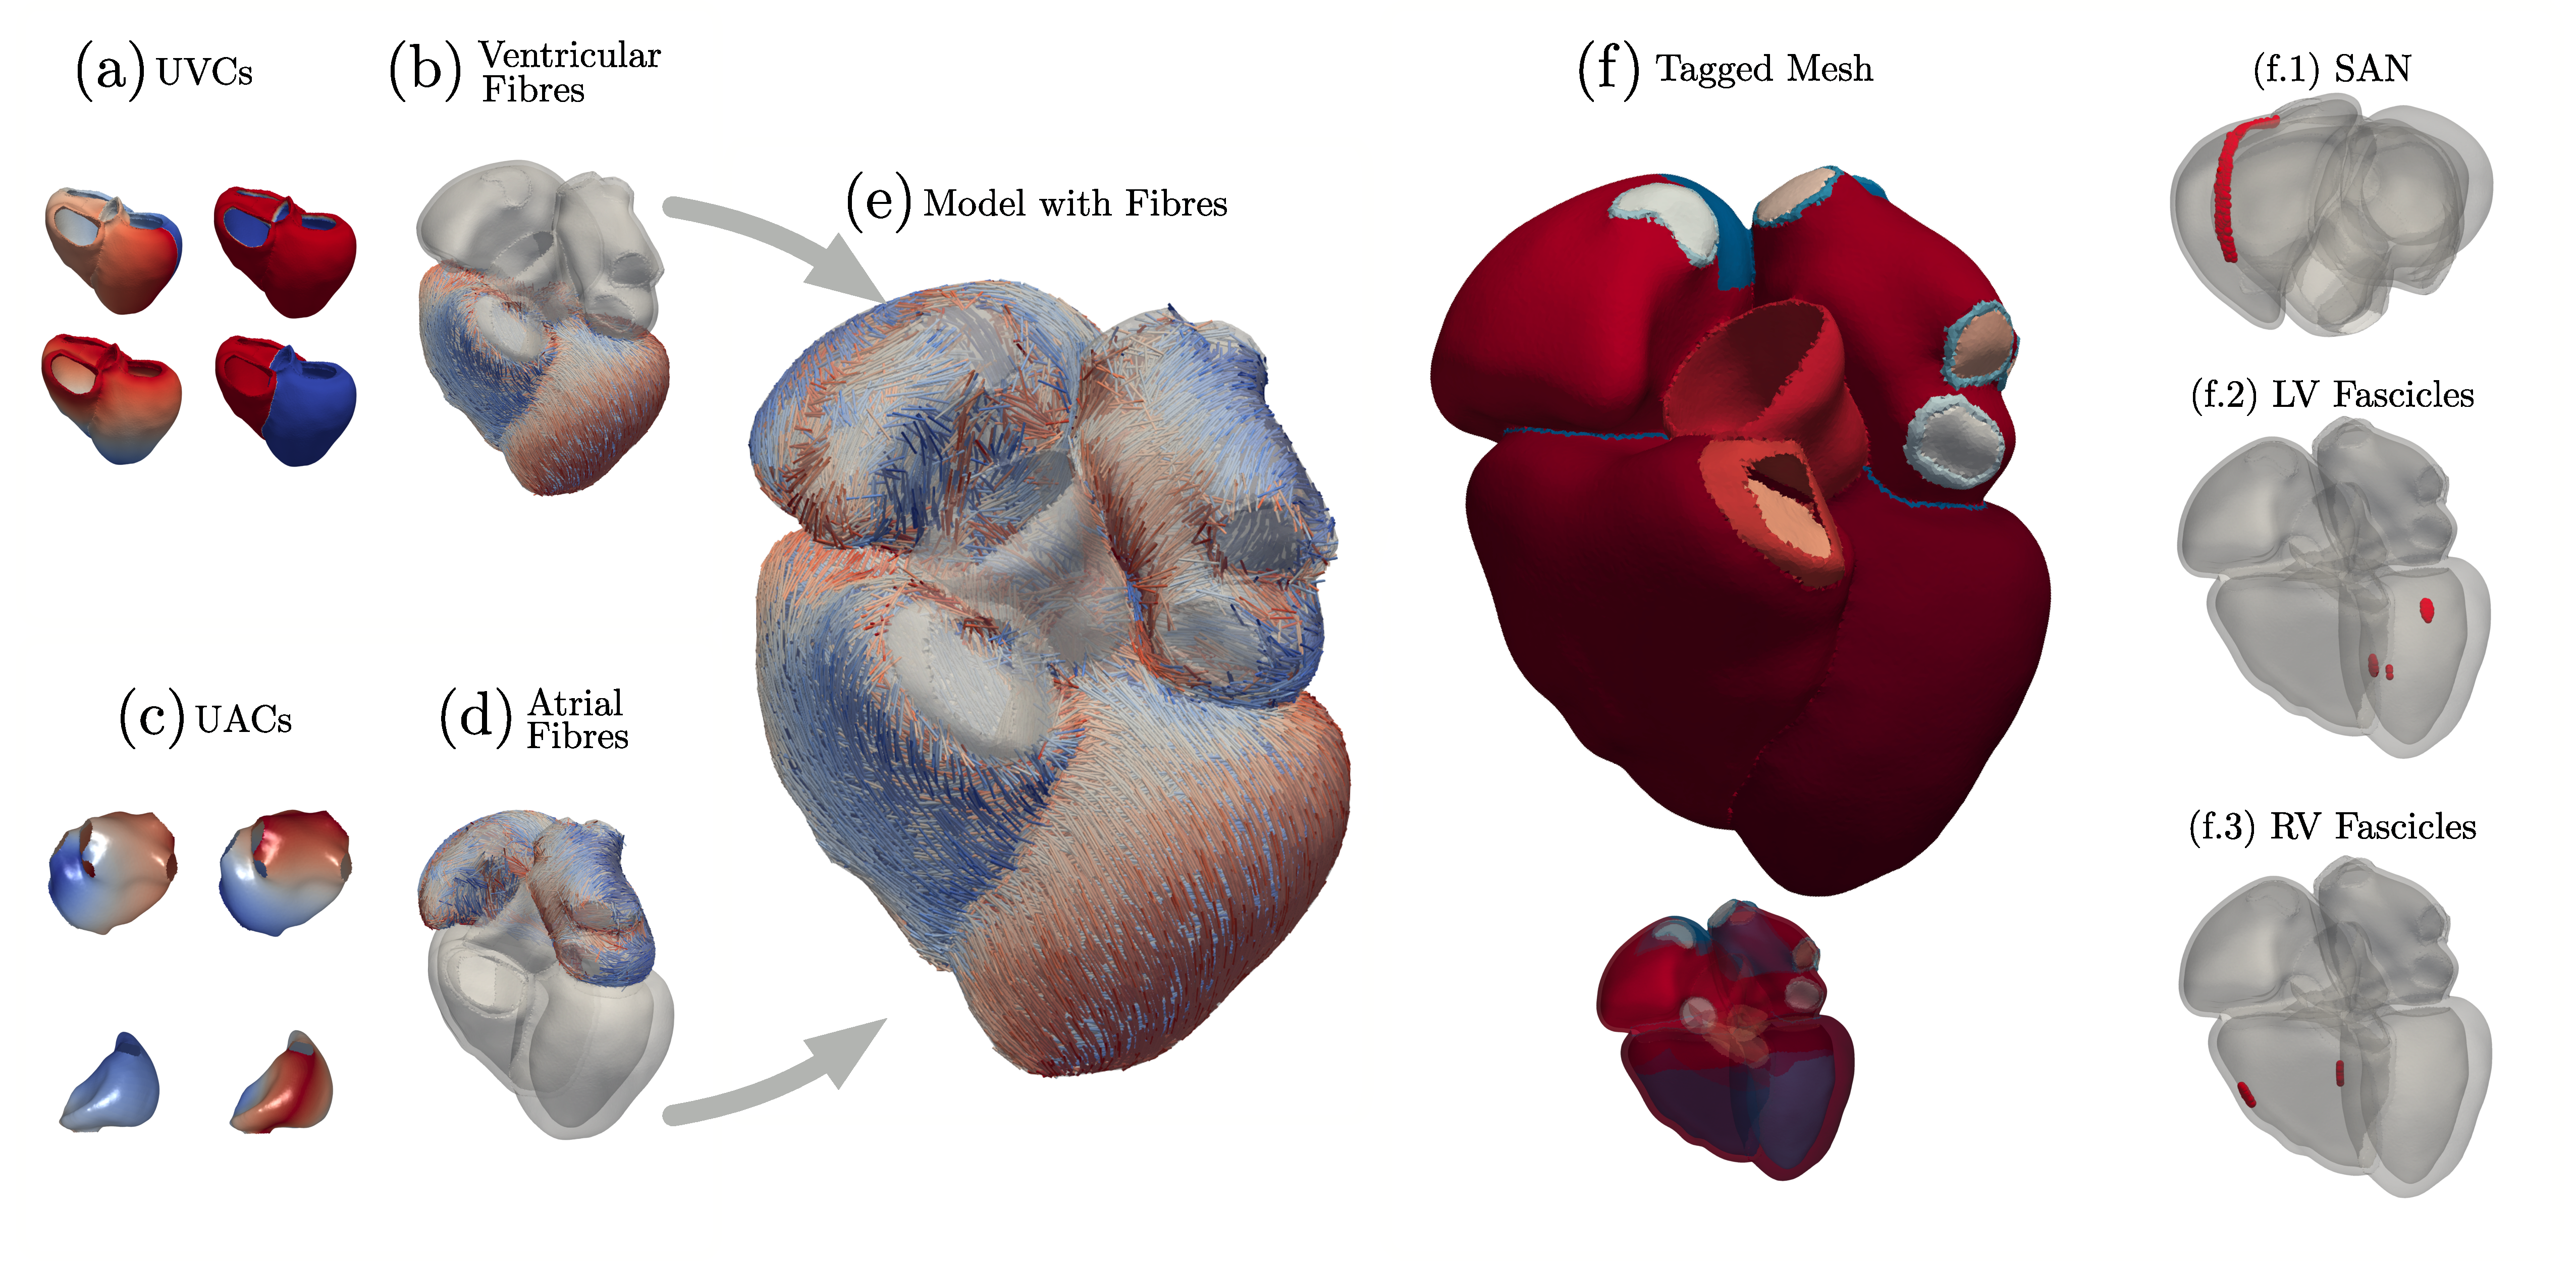
\includegraphics[width=\linewidth]{Fig4}
    \caption[Model creation stage. ]{
        \textbf{Model creation stage. }
        % Description of UVCs and ventricular fibres:
        Universal Ventricular coordinates (a) are calculated from the mesh, then used to assign 
        the fibre direction (b) using a rule-based algorithm~\cite{bayer2012_fibres}.
        % Description of UACs, atrial fibres, and mapping them to 3D:
        Universal Atrial coordinates (c) are calculated from the mesh, then used to assign
        the fibre direction (d) using a projection from an atlas~\cite{Roney2021-atlas}.
        The atrial fibres, which originally are produced on surfaces, are then projected onto the 3D
        mesh.
        % Tags, electrodes and FEC layer 
        The fibres from the ventricles and atria are then assigned to the model (e).
        The final mesh is tagged with the different labels needed for the simulations (f).
        The fast endocardial conduction layer (FEC) is also created at this stage (f~-~bottom),
        which is a thin layer of fast conducting tissue at the endocardium of the ventricles.
        Finally, UVCs and UACs are used to create the sino atrial node (\SAN, f.1),
        the left ventricle fascicles (f.2) and right ventricle fascicles (f.3).
    }
    \label{fig:methods-model-creation}
\end{figure}

\subsection{Simulations}\label{sec:simulations}

We performed EP and mechanics simulations on all the models. 
Simulations were run with a fixed set of parameters to assess the impact 
anatomical differences would have on the outputs. 
These simulations also served as an additional quality check for the meshes, 
to ensure the models could be used to run electromechanics simulations. 

Each patient-specific mesh was simulated in its native 
coordinate system without spatial registration to a common anatomical 
reference frame. Comparisons between models were performed on scalar 
outputs (chamber volumes, total activation times) that are invariant 
to rigid transformations. Universal Ventricular Coordinates 
(UVCs)~\cite{bayer2018} provide normalized transmural and apicobasal 
coordinates for regional functional analysis independent of absolute 
spatial positioning.

The EP simulations were started at the \SAN, defined in Section~\ref{fig:methods-model-creation}. 
The ventricular endocardial electrodes (fascicles) were also activated simulating the early activation 
sites~\cite{Gillette-2021-dt}. 
The reaction-eikonal model~\cite{neic-2017-electrograms} was solved to compute the activation 
times at each node. 
A conduction velocity of $1$ m/s was used at the myocardial tissue, with a 
$40\%$ anisotropy cross-fibre, and a 
$6$-fold speed in the fast activation regions~\cite{lee-2019-fec}. 
As output, the total activation time of each ventricle, of both ventricles and both atria were extracted.

To test how differences in anatomy impacted simulation predictions,
we performed inflation simulations to evaluate the mechanical behaviour of the models.
Briefly, increasing pressure is applied at the endocardium of each chamber until a 
maximum established pressure of  
% 0.93~kPa for the left chambers (\LV\ and \LA) and
7~mmHg for the left chambers (\LV\ and \LA) and
% 0.466~kPa for the right chambers (\RV\ and \RA) 
3.5~mmHg for the right chambers (\RV\ and \RA) 
is reached.
The myocardium was modelled as an transversely isotropic hyperelastic material using the 
Guccione's material law~\cite{Guccione-1991-material-props}, 
while the rest of the cardiac structures were modelled as isotropic hyperelastic materials using a 
NeoHookean material law~\cite{faulkner-1972-nearly}. 
Mechanics simulations were run with the same boundary conditions as the work by~\cite{strocchi2023_cell}, 
which can be consulted in the Supplementary Material.

Simulations were run to assess the impact of anatomical differences on the outputs and to serve as 
a quality chech for the meshes. 
All simulations were run with CARP~\cite{carp-2003}. 
The EP simulations were run in a $20$-core workstation, 
while the inflation simulations were run in the UK national supercomputer ARCHER2, using $512$ cores.

% \subsection{Model Quality Control and Validation Tests}
Model outputs obtained from the simulations are listed in Table~\ref{tab:measurements},
along with a brief descripton. 
The 18 measurements are grouped into four categories:
activation times (4 outputs),
inflated volume (4),
volume change (absolute 4, and normalised 4), and
volume ratios (2).
The absolute volume change ($\deltaVol{}$) is calculated as the difference between the maximum and minimum volume
during the inflation simulation.
For simplicity, we refer to inflated volume as volume throughout the manuscript.
The normalised volume change ($\deltaVolNorm{}$) is calculated as the percentage of change in volume,
and the volume ratio is calculated as the ratio between the left and right volumes, 
this was calculated for the ventricles and the atria. 
The Total Activation Time ($\TAT{}$) is the time it takes for the electrical signal to propagate
through the entire chamber.

\begin{table}[hbpt]
    \centering
    \caption[Model outputs obtained from the simulations.]{
        \textbf{Model outputs obtained from the simulations.}
        The subscript $x$ refers to the chamber, which can be left ventricle (LV),
        right ventricle (RV), left atrium (LA), or right atrium (RA). 
    }
    \vspace{1em}
    \begin{tabular}{lll}
    \hline
    Measurement              & Symbol                           & Calculation / Definition                                                                                  \\
    \hline
    Total Activation Time    & $\TAT{x}$                        & All chambers, ventricles, and atria                                \\
    (Inflated) Volume        & $\VOL{x}$                        & All chambers                                                     \\
    Volume Change            & $\deltaVol{x}$                 & Maximum minus minimum volumes  \\
    Normalised Volume Change & $\deltaVolNorm{x}$            & Percentage of change in volume                  \\
    Volume Ratio             & $\frac{L}{R}$ & Ratio of left and right volumes \\                            
    \hline 
    \end{tabular}    
    \label{tab:measurements}
\end{table}

\paragraph{QRS duration.} 
Since the simulations do not include a torso, the comparison cannot be made directly 
with the QRS duration measured in the ECGs. 
Instead, we used the total activation time in the ventricles as a surrogate 
for QRS duration and compared it between the different groups.

\paragraph{Total Activation Time in the Atria.}
This parameter has emerged as a key marker of atrial remodeling and is associated with \HF\ 
progression and complications~\cite{sanders-2003-atrialremodelling,buck-2008-crt}.
We assessed the total activation time in the atria, comparing it between the different groups.

\subsection{Statistical tests and comparison of volume to clinical literature}
We performed a multi‐step statistical analysis of our cardiac dataset.
First, we computed descriptive statistics (mean $\pm$ SD) for all core metrics (volumes and activation times)
stratified by sex, condition (\HF vs. control), and subtype (\HFN vs. \HFW). 
% To assess mesh‐size validity, we calculated Pearson correlations between mesh element counts and activation times.
Differences between narrow and wide QRS durations are only explored qualitatively, as the number 
of cases in each group is low. 

\paragraph{Effect sizes and statistical significance.}
% You want to see if there's a difference in an outcome (e.g., a heart metric) depending on:
To assess the differences in the outcomes, we used a two-way ANOVA to test the effects of 
Sex, Condition, and their interaction.
We followed up significant ANOVA results in the interactions with post-hoc pairwise comparisons 
using Tukey's method, 
and calculated Cohen's $d$ effect sizes~\cite{cohen-2013-statistical} for each comparison.
If the interaction was not significant, we performed marginal comparisons
between \HF\ and controls, or male and female groups, across all cases.
% ADJUST FOR MULTIPLE COMPARISONS
P‐values were corrected for multiple comparisons using the Benjamini–Hochberg 
false discovery rate~\cite{Benjamini1995ControllingTF}. 
Effect sizes are reported as Cohen's $d$, 
using Gignac's expanded criteria~\cite{gignac-2016-effects},
where $d<0.5$ is small, 
      $0.5<d<0.8$ is moderate, 
      $0.8<d<1.2$ is large, 
  and $d>1.2$ is very large.
% Finally, we visualized group distributions via boxplots with overlaid swarm plots, and
% summarized effect sizes in forest plots. 

To externally validate the models, 
we compared different outputs from the pipeline % and from simulations and  
linked them to a clinically relevant metrics.

\paragraph{Left atrial and left ventricular volume.} 
Left atrial volume is a predictor of outcome in patients with chronic \HF, 
independently of their symptoms, age, or \LV\ function~\cite{rossi-2007-lav}. 
\LV\ volume is a key prognostic factor in \HF, 
as it is associated with the severity of the disease and the risk of 
adverse events~\cite{kasa-2024-lv_volume,ito-2021-lv_volume}.
We assessed the left atrial volume ($\VOL{LA}$) and \LV\ volume ($\VOL{LV}$) in the models, 
comparing between the different groups.
For $\VOL{LV}$, we compared measurements from our cohort with reference values from the UK biobank 
(UKBB)~\cite{petersen-2017-reference}, which defines normal ranges for left and right ventricles
in males and females. 
Outside the normal ranges, we considered the volumes to be abnormal,
and therefore indicative of \HF\ or other cardiac conditions. 

% \paragraph{Left-ventricular and left-atrial chamber stiffness.}
% Stiffness can be approximated in a shell with constant thickness using Laplace's law.
% It is measured as the ratio between change in pressure and change in volume. 
% In our simulations, as the pressure is always the same for all cases, 
% the change in volume becomes a surrogate for stiffness. 
% It has been reported that patients  with \HF\ show increased 
% \LV\ chamber stifffness~\cite{zile-2004-stiffness,aurigemma-2006-stiffness}.
% Similarly, \LA\ chamber stiffness has shown to predict mortality and 
% hospitalisation~\cite{Carpenito-2021-la-stiffness,kim-2023-la-stiffness}. 
% Because stiffer chambers deform less under the same pressure, increased volume change ($\deltaVol{LV}$) 
% indicates reduced chamber stiffness. 
% Therefore, if chamber stiffness is reduced in the heart failure group, 
% we expect to observe a larger volume change compared to controls.



% 
% --- end input:   sections/methods ---


% --- begin input: sections/results_final ---
\section{Results}
Fifty whole-heart models
\replaced[id=PLOS, comment={Reviewer: cohort overview figure moved to supplement; cited as S1 Fig.}]{(\ref{fig:s1-hearts} Fig)}{(Figure~\ref{fig:hearts})}
were created, each including EP and mechanics simulations described in Section~\ref{sec:simulations}.
All simulations were performed with the same parameters for each model.
Therefore, the differences in simulations between sexes reported below relate to 
differences in anatomy.
% \paragraph{Descriptive statistics.}
We first examined the distributions of all core metrics across sex and condition.
A full table of means and standard deviations is provided in the Supplementary Material.
We found no significant difference in age between males and females
(M: $53.4\pm15.0$\,y; F: $54.6\pm10.7$\,y; $p=0.75$). 
% % supplementary material: summary_table.xlsx 

\paragraph{Geometric characterization and correlation with simulation outputs.}
Geometric metrics stratified by sex and condition are provided in 
\replaced[id=PLOS, comment={PLOS: S1 Table form}]{\ref{tab:s1-geometric-characteristics} Table}{Supplementary Table~\ref{tab:s1-geometric-characteristics}}. 
Heart failure patients exhibited substantially larger chamber volumes 
compared to controls, with male HF patients showing the most pronounced dilation 
(LV: $289 \pm 88$~mL vs control: $180 \pm 36$~mL, $p<0.001$). Myocardial wall 
volume scaled with anatomical size, ranging from $263 \pm 37$~cm$^3$ 
in female controls to $396 \pm 75$~cm$^3$ in male HF patients.

Geometric variables showed strong correlations with simulation outputs 
(\replaced[id=PLOS, comment={PLOS/REV: S3 Fig (renumbered after hearts moved to S1)}]{\ref{fig:s3-correlation-heatmap} Fig}{Supplementary Figure~2}).
Chamber volume was the strongest predictor of 
volume change during passive inflation ($\rho = 0.96$ for LV, $p < 0.001$), 
indicating that larger ventricles exhibit greater absolute compliance under 
uniform material properties. Myocardial wall volume correlated strongly with 
activation times ($\rho = 0.87$ for TAT$_{\mathrm{RV}}$, $\rho = 0.85$ for 
TAT$_{\mathrm{V}}$, both $p < 0.001$), reflecting the expected increase in 
conduction path length with anatomical size. Notably, cross-chamber geometric 
correlations were observed, such as RV volume predicting LV activation time 
($\rho = 0.81$, $p < 0.001$), consistent with whole-heart anatomical coupling.

% Reviewer request: cohort overview figure (fig:hearts) moved to supplement as S1 Fig.
% See sections/supp/s_fig1_hearts.tex; label is now fig:s1-hearts.


% \subsection{Clinical literature metrics.}
Next, we assessed model volumes and the outputs of the EP and mechanics simulations.
In each case, we report the results from the two-way ANOVA and the post-hoc tests, showing 
the effect sizes. 
Where no interaction was present, we examined independent effects.
In both cases, only statistically significant results after FDR correction are reported here.
Effect sizes were computed using Cohen’s $d$ and are visualised in 
\replaced[id=PLOS, comment={PLOS: Fig (no period)}]{Fig}{Figure}~\ref{fig:cohen-big-effects}.

% \paragraph{\LA volume.} $\VOL{LA}$ had a significanfly higher mean in \HF\ patients,
\paragraph{\LV\ volume.} 
$\VOL{LV}$ was significantly larger in \HF\ patients and showed a significant interaction 
($p<0.05$ in ANOVA and all post-hoc comparisons).
For all but three male controls, the \LV\ volumes fall within the normal range 
($[109,218]$~mL)
compared to the UKBB reference values~\cite{petersen-2017-reference}.
Similarly, female controls also fall mostly within their corresponding normal range
($[88,161]~mL$).
We display the results in \replaced[id=PLOS, comment={PLOS: Fig (no period)}]{Fig}{Figure}~\ref{fig:validation-volumes}.
The effects sizes were also large between \HF\ and control groups, but they were much 
larger in males than in females, for instance, 
interactions involving females ranged between $0.9<d<1.17$, 
while interactions involving males were higher than $d>1.4$ 
($p<0.05$ in all cases, \replaced[id=PLOS, comment={PLOS: Fig (no period)}]{Fig}{Figure}~\ref{fig:cohen-big-effects}(a)).

\begin{figure}[hbpt]
    \centering
    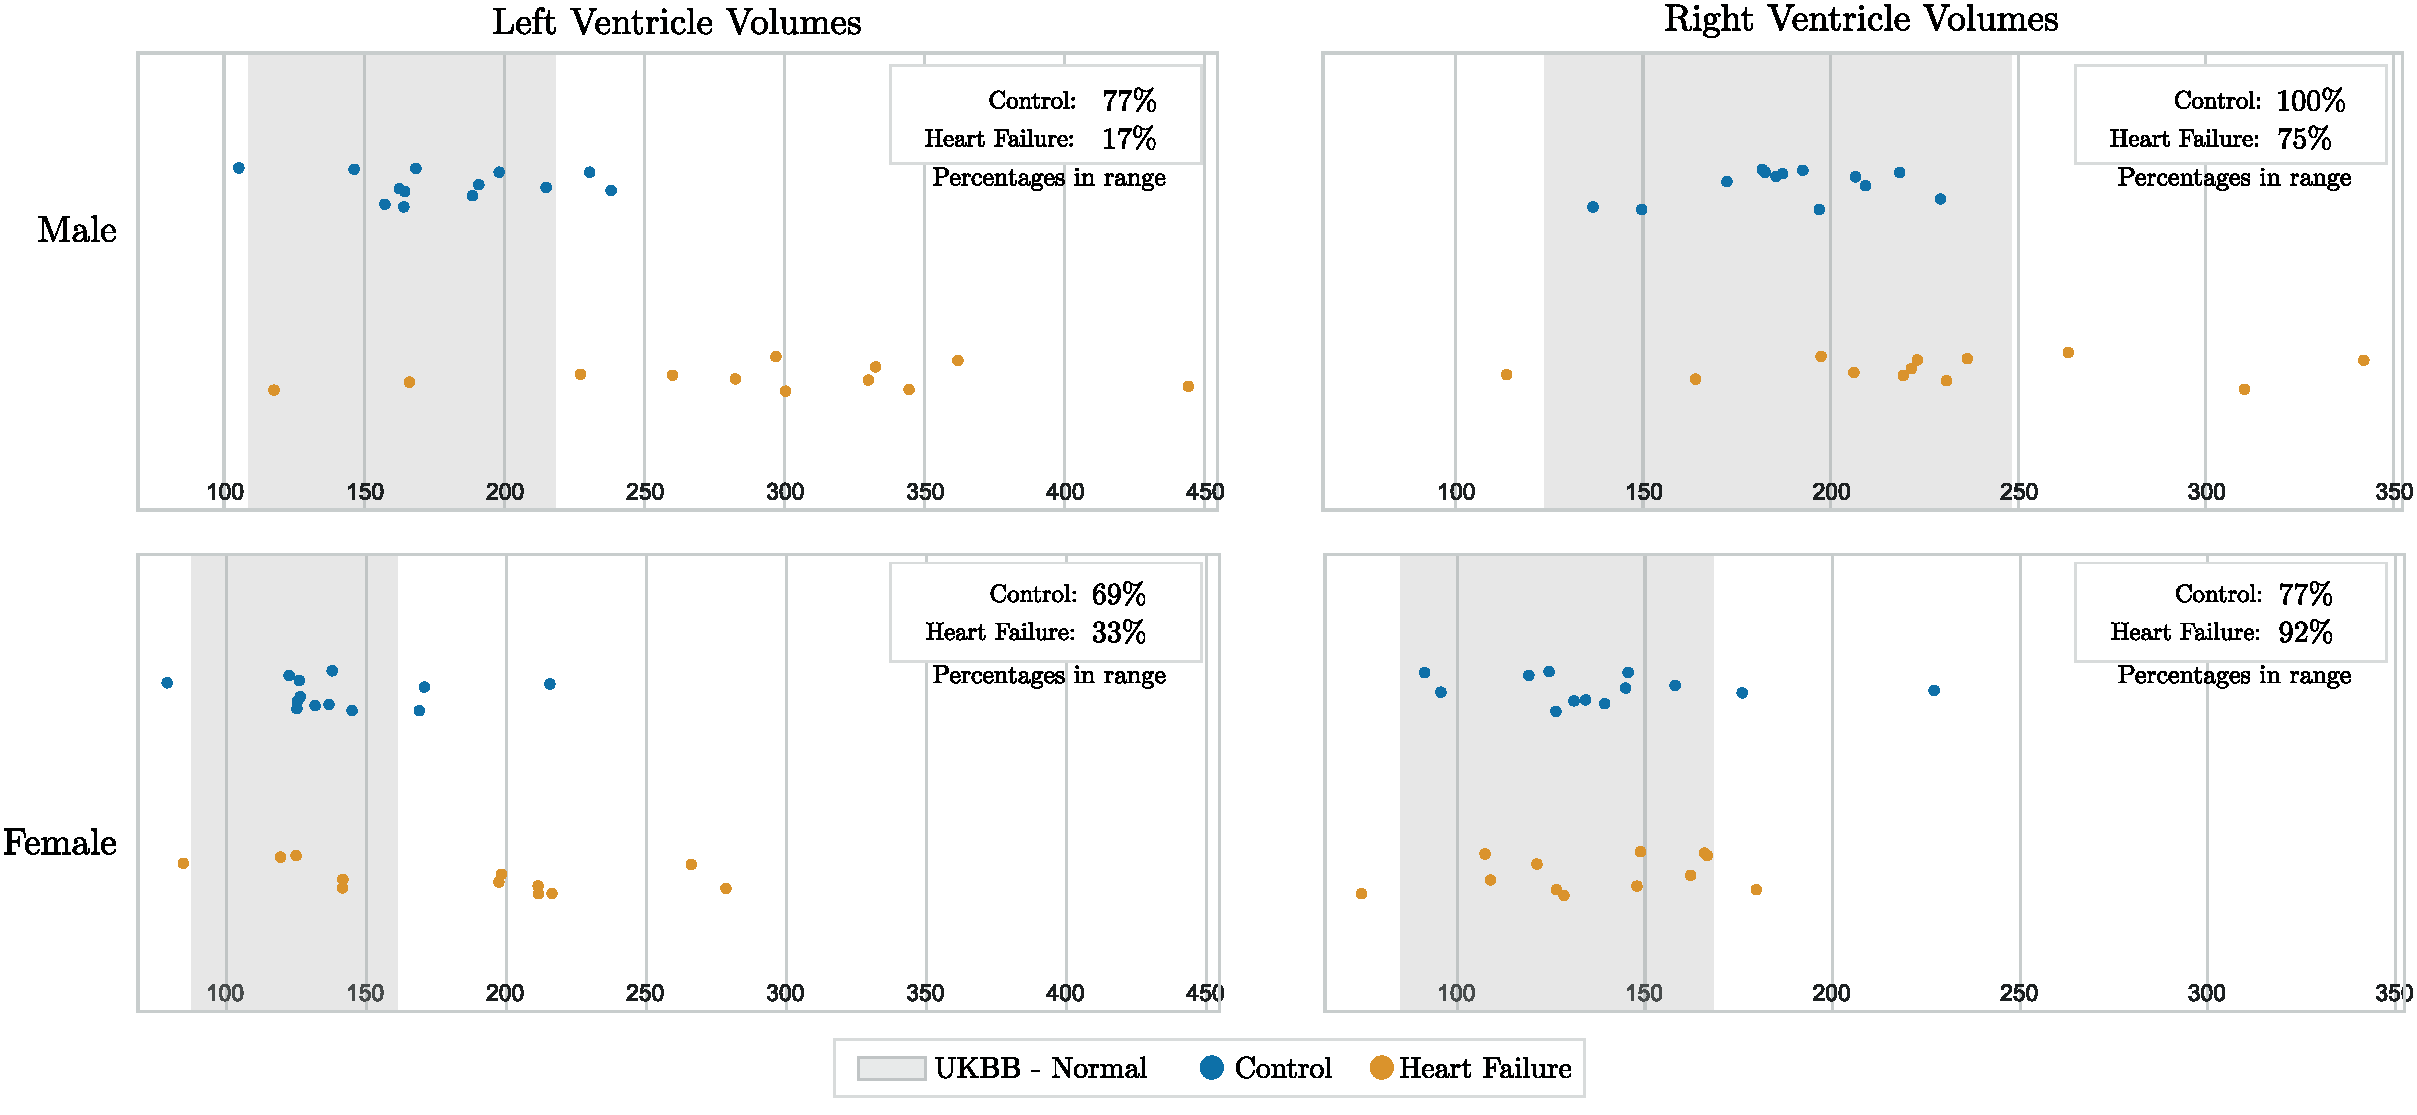
\includegraphics[width=\textwidth]{Fig5}
    \caption[Comparison vs clinical literature values and ranges from UKBB.]{
        \textbf{Comparison of measured ventricle volumes from the virtual cohort with}
        clinical literature values and ranges from UKBB.
        The UKBB normal ranges are defined as measurements within the 95\% prediction interval
        of the study by~\cite{petersen-2017-reference}. 
        Two graphs, corresponding to the \LV\ and \RV\ metrics and reference volumes. 
        Each plot is separated by sex and coloured by condition, with Controls in blue and 
        Heart Failure in orange.
        Normal ranges are shown as greyed areas, and exceeding the upper limit of the
        reference range may indicate pathological ventricular dilation. 
        Percentages of each group within the UKBB normal range are displayed in the legend.
    }
    \label{fig:validation-volumes}
\end{figure}
% ()
\paragraph{Volume change in the \LV.}
We used volume change as a surrogate for stiffness. 
\LV volume change was significantly larger in males compared to females and in 
\HF\ patients compared to controls (both main effects with $p<0.01$), 
but we did not detect a significant sex~$\times$~condition interaction ($p=0.44$), 
indicating that sex and condition contribute independently to \LV\ volume change. 
The effect sizes were large, with $d=0.94, p<0.01$ for \HF\ vs controls, 
and $d=0.78, p<0.01$ for male vs female comparisons 
(\replaced[id=PLOS, comment={PLOS: Fig (no period)}]{Fig}{Figure}~\ref{fig:cohen-big-effects}b).

\paragraph{Activation times.}
For ventricular $\TAT{V}$, no significant interaction was found between sex and condition ($p=0.76$), 
however, the independent effect sizes were large. 
First, $\TAT{V}$ was significantly longer in males compared to females ($d=1.4, p<0.01$), 
and in \HF\ patients compared to controls ($d=0.72, p=0.014$).
$\TAT{LA}$ showed a similar pattern. First, no significant interaction between sex and condition 
was found ($p=0.24$). Second, the independent effects were significant and moderate, showing 
prolonged activation times in \HF\ vs. controls ($d=0.62, p<0.05$) and prolonged activation 
in males vs. females ($d=0.59, p<0.05$). 

To assess the validity of using \TAT{} as a surrogate for QRS 
duration in the absence of torso modeling, we correlated simulated ventricular 
\TAT{} with recorded ECG QRS duration in cases where ECG data were available 
($n=33$ of $50$). In control hearts, \TAT{} showed a positive correlation with 
QRS duration (Pearson $r = 0.649, p < 0.005$, 
\replaced[id=PLOS, comment={PLOS/REV: S2 Fig (renumbered after hearts moved to S1)}]{\ref{fig:s2-tat-qrs} Fig}{Supplementary Figure~1}),
indicating that simulations using reference conductivity parameters provide an 
approximate anatomical surrogate for QRS duration, and that anatomical variation 
captures at least part of the inter-subject variability in activation time. 
In heart failure patients, no correlation was observed ($r = -0.127, p = 0.64$), 
consistent with the expected influence of pathological tissue properties 
(fibrosis, conduction blocks) that are not represented in our standardised 
parameter set.

\paragraph{Normalised volume changes in \LV.}
$\deltaVolNorm{LV}$ showed a significant interaction in the ANOVA between sex and condition ($p<0.05$).
Post-hoc tests only showed effects sizes were significant when comparing
\begin{itemize*}
    \item[] Male \HF\ vs. male controls ($d=-1.33$),
    \item[] Male vs. female with \HF\ ($d=-1.09$),
\end{itemize*} 
both with $p<0.05$.

% The largest effects were consistently observed in the ventricular metrics, 
% particularly in right ventricular volume and activation time between sexes, and in 
% left ventricular volume between males with and without heart failure.

\begin{figure}[hbpt]
    \centering
    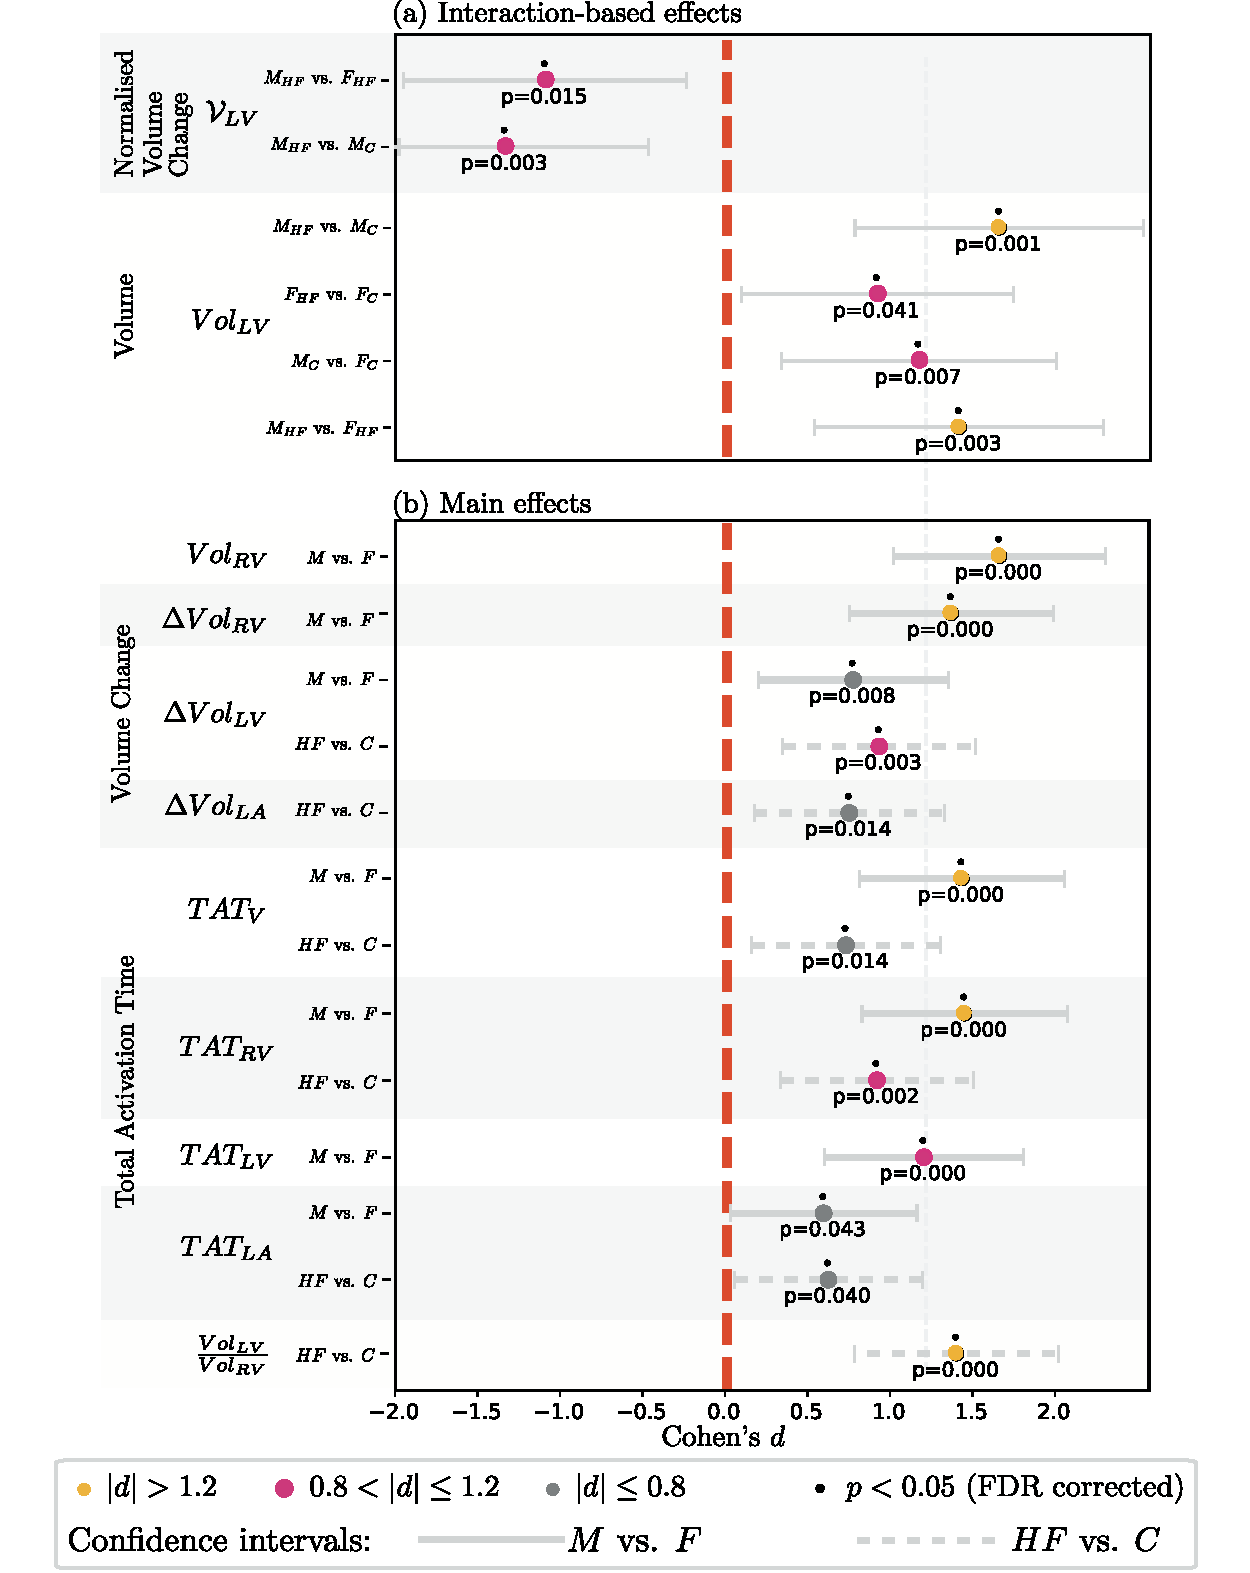
\includegraphics[width=\linewidth]{Fig6}
    \caption[Large effect sizes from post-hoc comparisons.]{
        \textbf{Cohen’s d effect sizes from post-hoc comparisons following two-way ANOVA.}
        Metrics and group comparisons are displayed on the y-axis.
        This graph only shows effects with a high effect size and a corrected p-value $p<0.05$. 
        (a) Effect sizes for group comparisons performed when the Sex~$\times$~Condition 
        interaction was statistically significant, justifying 4 simple-effect post-hoc tests.
        (b) Effect sizes for marginal comparisons, when no significant interaction was found.
        Error bars line styles represent the comparison made: solid for sex, dotted for condition.
        \textit{Abbreviations}: M=Male, F=Female; C=Control, HF=Heart Failure; TAT=Total Activation time, 
        L/R=Left/Right, V=Ventricle.
    }
    \label{fig:cohen-big-effects}
\end{figure}
% --- end input:   sections/results_final ---


% --- begin input: sections/discussion_final ---
\section{Discussion}
% 1. summarise what we have shown.
We created a sex-balanced virtual cohort of 50 whole-heart models derived from clinical CT scans of 
both healthy individuals and \HF\ patients. 
We used a semi-automated pipeline to generate these models,
which includes segmentation, mesh generation, fibre orientation assignment, and simulation setup.
The models enabled the exploration of differences in volume, and activation time across sex and disease groups, 
using benchmark electrophysiology and mechanics simulations. 
With this study, we demonstrate that anatomical differences between sexes and across disease states have a 
significant impact on both electrical and mechanical simulation predictions in the heart. 
This highlights the critical need to account for such variations when developing and 
applying computational models in cardiology.

% 2. comment on other workflows
A variety of computational pipelines have been proposed to construct heart models, 
ranging from atria-only or ventricles-only representations to anatomically detailed four-chamber reconstructions.
The works by~\cite{roney-2023-atriamodels} and~\cite{azzolin-2023-atriamodels} proposed 
patient-specific atrial models, including anatomical regions and fibre orientations from clinical data.
In contrast, other pipelines focus only on ventricular chambers~\cite{govil-2023-bivmodels,banerjee-2021-bivmodels}.
A notable whole-heart model was developed by~\cite{zhang-2012-fourchmodels}, 
which builds detailed four-chamber meshes of the entire heart from patient imaging and has been enhanced 
since to improve 
simulation fidelity, 
multi-scale integration, and 
clinical translation.
The resulting models are anatomically detailed, but the method depended on extensive user guidance to 
create the initial atlas, limiting throughput and scale.
Other groups, such as Gillette et al.~\cite{gillette_personalized_2022}, have also 
demonstrated personalised whole-heart electrophysiology models, but again with 
significant manual setup and typically small cohorts.

In summary, existing pipelines either produce atria-only or ventricle-only models, 
or else deliver high-detail four-chamber meshes at the cost of manual effort.
Our framework seeks to overcome these limitations by producing anatomically complete four-chamber 
(atria + ventricles) models with minimal manual input, combining scalability with high anatomical fidelity.

\subsection{Building Patient-Specific Whole-Heart Models: Workflow Insights}
The models were created using a standardised pipeline, CEMRG heartbuilder, 
which allows for the generation of patient-specific models from CT scans. 
The segmentation framework has enabled a substantial reduction in overall model generation time relative to 
earlier methods. The pipeline requires approximately 5 hours per heart on average.
It is also significantly more detailed than most publicly available pipelines. 
For instance, methods evaluated in the MICCAI 2024 Whole Heart Segmentation Challenge~\cite{miccai2024_challenge} 
typically produce 7–10 output labels, insufficient for physiologically realistic biophysical simulations. 
In contrast, our approach employs a 37-label standard~\cite{strocchi2020_cohort,strocchi2020_simulating}, 
encompassing detailed delineation of blood pools, myocardia, valve planes,
and major vessels across all four chambers.

The current implementation applies uniform meshing parameters globally 
across the whole heart. While regional refinement could theoretically be 
achieved by meshing structures separately and stitching at interfaces, 
we prioritized mesh integrity to ensure numerical stability in coupled 
electromechanical simulations, where interface discontinuities can 
introduce artifacts.

The strong correlations between geometric metrics and simulation outputs 
(\replaced[id=PLOS, comment={PLOS/REV: S1 Table / S3 Fig (renumbered after hearts moved to S1)}]{\ref{tab:s1-geometric-characteristics} Table, \ref{fig:s3-correlation-heatmap} Fig}{Supplementary Table~1, Figure~2}) demonstrate that anatomical variability
is a primary driver of functional differences when using standardized 
electrophysiological and mechanical parameters. Chamber volume alone explained 
92\% of variance in volume change during inflation ($\rho = 0.96$), indicating 
that anatomical size dominates mechanical behavior under uniform constitutive 
laws. Similarly, myocardial wall volume predicted 76\% of variance in right 
ventricular activation time ($\rho = 0.87$, $p < 0.001$), consistent with 
total myocardial mass determining conduction path length and duration.

These findings validate our approach of isolating anatomical effects through 
parameter standardization. However, they also highlight the limitation: 
real-world patient-specific predictions would require calibration of tissue 
properties (contractility, stiffness, conduction velocity) to observed 
clinical metrics.

% \subsection{Discussion on the results}
\subsection{Impact of Anatomical Variability on Electromechanical Predictions}
All whole-heart models were simulated using identical parameters for both electrophysiology and mechanics. 
% This design choice ensured that any inter-group variation in simulation output arose solely from 
% differences in anatomy, rather than from parameter fitting or model calibration. 
We did not include active contraction in the benchmark as these simulations often require patient specific 
parameters to match contraction, pre-load and after load, 
reducing our ability to compare consistent simulations across anatomies.
As such, the results reflect the isolated impact of anatomical structure variation
due to sex or disease status on predicted electrical activation and mechanical inflation.
The results from the two-way ANOVA showed, in most cases, non significant interactions.
This means that we could only look at the independent effects: control vs \HF\ and 
male vs female. 
The characterisation of effect sizes (small, moderate, and large) by~\cite{gignac-2016-effects}, 
were included as a guideline, based on the distribution of effect sizes obtained.

\subsection{Comparison with Clinical Reference Ranges}
Comparison with population-based MRI reference data~\cite{petersen-2017-reference} 
demonstrated that control models reproduced expected sex-specific chamber sizes, 
serving as an anatomical fidelity check for our reconstruction pipeline. 
Male and female \LV\ and \RV\ volumes were largely consistent with normal ranges, 
supporting the accuracy of our segmentation and meshing workflow. 
However, because mechanical simulations used uniform material properties across all cases, 
the observed volumes represent anatomical structure rather than patient-specific functional state. 
In heart failure, \LV\ enlargement was most pronounced in males, frequently exceeding 
reference thresholds, consistent with classical patterns of systolic dilation. 
Females also showed increased \LV\ volumes, though these remained mostly within upper limits, 
highlighting sex differences in disease expression. 
\RV\ enlargement was less prominent in both males and females with HF, 
reflecting clinical reports that \RV\ size is less sensitive to early disease~\cite{ro-2023-rv_volume}. 
These results demonstrate that the virtual cohort captures both healthy anatomy and 
pathological remodeling patterns at the population level.


\paragraph{Impact of Sex and Heart Failure in \emph{In-Silico} Studies}
Our simulations consistently separated groups by sex and disease status using 
uniform electrophysiological and mechanical parameters, demonstrating that 
anatomical variability alone produces measurable functional differences. 
When population-level material properties are applied to pathological geometries, 
the resulting simulations capture group-level trends consistent with clinical observations. 
Absolute LV volume increases were particularly marked in male HF, reproducing the 
clinical signature of pathological dilation~\cite{kasa-2024-lv_volume,ito-2021-lv_volume}. 
Larger $\deltaVol{LV}$ in HF models reflects the mechanical consequence of dilated 
geometry under uniform compliance parameters~\cite{zile-2004-stiffness,aurigemma-2006-stiffness}. 
Similarly, larger $\deltaVol{LA}$ patterns align with clinical markers of atrial 
dysfunction~\cite{Carpenito-2021-la-stiffness,kim-2023-la-stiffness}. 
When expressed as normalized change      
(\replaced[id=PLOS, comment={PLOS: Fig (no period)}]{Fig}{Figure}~\ref{fig:cohen-big-effects}a), 
however, \HF\ females showed the greatest relative differences, 
driven by smaller baseline chamber sizes. 
This emphasizes that absolute and relative measures provide complementary insights in 
sex-stratified analyses~\cite{steuernagel2023_sex_bias}. 
Electrical activation followed similar patterns: ventricular and atrial activation were 
prolonged in HF and in males, consistent with clinical QRS and conduction 
observations~\cite{sanders-2003-atrialremodelling,buck-2008-crt}. 
These convergent trends highlight that population-level simulations with anatomically 
accurate models can reproduce group-level clinical patterns, while individual patient 
predictions would require tissue-specific parameter calibration~\cite{strocchi2020_cohort}.


\subsection{Establishing Model Credibility and Validation Strategies for In Silico Clinical Trials}
In silico studies using virtual cohorts of patients, referred to as in silico clinical trials (ISCTs), 
require careful demonstration of model credibility for their conclusions to be considered reliable. 
Credibility is primarily established by performing validation, that is, comparison of model predictions 
with real-world data. 
However, unlike relatively simple models of standalone medical devices, or drug safety/efficacy studies 
using a generic action potential model, ISCTs present a much wider range of possible validation strategies. 
As discussed in detail in~\cite{pathmanathan-credibility-2024}, possible evaluation activities include: 
validation of a device/drug model in isolation 
(e.g., bench test validation of a pacemaker lead mechanics model); 
individual-level validation of patient models in the cohort 
(i.e., comparing predictions from a specific patient model with clinical data from the specific patient 
the model represents), 
population-level validation of the cohort or sub-cohorts 
(e.g., comparing the distribution of model outputs across the cohort with clinical data from the 
corresponding real-world population), 
validation of coupled device-patient or drug-patient models 
(e.g., PKPD validation studies), 
and validation of any statistical model used to convert patient model outputs into clinical endpoints. 
Also, there are important additional activities that should be performed, such as assessing the virtual 
cohort representativeness; 
these are not strictly model validation activities and more akin to model input validation for 
simple models.
 
Overall, an ISCT is expected to be supported by a body of evidence on model credibility. 
For a virtual cohort such as the sex-balanced 50 patient cohort provided here, 
intended for re-use in variety of future device or drug ISCTs, 
a hierarchical evaluation approach can be used to generate an initial body of credibility evidence 
to support a future ISCT.

In this work, we have conducted a preliminary assessment of anatomical representativeness 
by comparing ventricular and atrial volumes in the male and female cohort subsets with 
corresponding UK BioBank data. This comparison demonstrates that our reconstruction pipeline 
accurately captures population-level anatomical distributions, establishing a foundation 
for future credibility assessments. However, full validation for in silico clinical trials 
would require additional hierarchical evaluation steps, including patient-specific 
functional validation, uncertainty quantification, and context-specific device or drug 
interaction studies~\cite{pathmanathan-credibility-2024}.
 
A natural next step would be to perform sex-specific population-level validation: 
demonstrating that the distribution of model outputs, for each of the male and female sub-cohorts, 
match the distribution observed in the male and female populations, 
particularly for outputs for which a statistically significant sex difference was observed. 
For instance, predicted chamber $\TAT{}$ distributions could be compared with sex-specific population 
QRS duration data, 
after an appropriate transformation to account for the fact that $\TAT{}$ is only a surrogate for QRS.
Individualized validation, while more challenging, could be performed for newly generated patient models.
Ultimately, these results would be supplemented by context-specific validation when the cohort is used in a 
device/drug ISCT, together with other credibility assessment activities such as verification and 
uncertainty quantification~\cite{health_assessing_2023}.

\subsection{Limitations}
This work has four main limitations that should be considered when interpreting the results.
% + sample size 
First, the small sample size within each category of \HF , narrow and wide QRS duration, 
limits the statistical power for detecting subtle effects or interactions. 
Nonetheless, by balancing sex and \HF\ subtype, our dataset offers a structured 
starting point for exploring sex-disease interactions in-silico.
Furthermore, it can serve as a foundation for synthetic cohort 
generation~\cite{rodero-2021-virtualcohort1000,rodero-2021-virtualcohortextreme}
with a more diverse range of anatomical and clinical characteristics. 
% + complex simulations
Secondly, the simulations performed in this work were benchmark simulations 
% + parameters not calibrated 
and the parameters were not calibrated to the individual anatomies.
However, the use of a common set of parameters across all cases
ensured that the differences observed in the results were purely anatomical.
% time spent on the pipeline
Third, the pipeline requires 5 hours per heart on average, 
with 2 hours spent performing manual corrections required at the segmentation stage.
Even so, this is a significant reduction compared to previous methods.
Finally, limitations remain at the segmentation stage. 
Because this step underpins all subsequent model construction, 
we discuss its implications in more detail in the following section.

Our simulations employed uniform electrophysiological and 
mechanical parameters across all models to isolate the effects of anatomical 
variability. The positive correlation between simulated activation times and 
QRS duration in control hearts ($r=0.649, p<0.005$) indicates that reference 
conductivity parameters provide an approximate anatomical surrogate for QRS, 
and that anatomical variation captures at least part of the inter-subject 
variability in conduction time. It does not, however, constitute a precise 
prediction of QRS, nor does it account for patient-specific tissue properties 
such as fibrosis or conduction system disease. The absence of correlation in 
heart failure patients ($r=-0.127, p=0.64$) reflects this limitation and 
highlights the need for patient-specific parameter calibration.

Additionally, the UKBB reference ranges used for anatomical 
comparison~\cite{petersen-2017-reference} were derived from a predominantly 
Caucasian population. Ethnicity data were not systematically collected for the 
present cohort, which is consistent with common clinical practice in 
Europe~\cite{reporting_ethnicity_2004}, but may limit the generalisability of 
comparisons with these reference ranges for non-Caucasian patients. Racial 
differences in cardiac structure and function have been 
reported~\cite{effect_on_race_2019}, underscoring the importance of 
ethnicity-matched reference data when assessing anatomical fidelity in 
diverse cohorts.

\subsubsection{Critical Role of Segmentation in Model Accuracy}
The segmentation stage is a critical bottleneck in the pipeline,
requiring notable manual input to ensure anatomical fidelity.
The most frequent issues involve small gaps or discontinuities in the myocardium, 
where the wall becomes excessively thin.
The segmentation method proposed by~\cite{hao2021_ccta} is not robust against some artefacts
introduced by implanted devices, such as the bright streaks caused by leads or stents in \HF\ patients. 
Manual steps and corrections in the pipeline could potentially be replaced with more 
robust algorithms. 
For example, recent work by~\cite{qayyum-2025-foundationmodel} demonstrated a 
foundation model capable of deriving full myocardial masks without user input.
Finally, given the limited soft-tissue contrast and resolution of standard CT scans, 
the myocardial thickness in chambers outside of the \LV\ is set to a user-specified constant.
This approximation may not reflect the true myocardial thickness 
and may underestimate simulation variability.

Full voxel-level correspondence assessment of the 37-label post-processed 
geometry against clinical images is not feasible for this dataset: CT 
soft-tissue contrast does not resolve myocardial boundaries outside the \LV, 
and structures including the \RV\ wall, atria, and great vessel walls are 
assigned thickness via distance maps at a user-specified constant. 
For the 10-label segmentation stage, geometric accuracy is supported by the 
published validation of the deep learning model~\cite{hao2021_ccta}. 
Population-level consistency of chamber volumes with \UKBB\ reference 
ranges (Section~\ref{sec:simulations}) provides indirect geometric 
plausibility evidence at the cohort level.

\subsubsection{Uncertainty Quantification}\label{sec:uq}
This study addresses variability across the population — how anatomical 
differences between patients influence simulation outcomes under fixed 
parameters. A distinct and equally important source of variability arises 
during model construction, introduced through segmentation choices and 
boundary placement. Previous work has begun to quantify this 
construction-stage uncertainty in the context of left atrial 
models~\cite{solis-lemus2023_reproducibility, sim2019reproducibility}, 
demonstrating that operator variability in segmentation introduces 
quantifiable differences in chamber geometry and downstream simulation 
predictions. However, whole-heart models present substantially greater 
complexity, with four chambers, multiple vessel junctions, and valve planes 
that may amplify uncertainty propagation through the reconstruction workflow. 
Explicitly quantifying construction-stage uncertainty in whole-heart models 
has not been addressed here and represents an important limitation, 
particularly in the context of regulatory credibility frameworks such as 
those outlined by the FDA~\cite{health_assessing_2023}.

Despite these limitations, our current approach balances physiological realism with scalability, 
enabling whole-heart simulations across a sizeable cohort. 
Incorporating more refined fibre estimation methods remains an important direction for improving 
predictive accuracy in personalised cardiac models.
By incorporating this level of anatomical detail into a reproducible, Python-based workflow, 
our pipeline bridges the gap between clinical image segmentation and simulation-ready models. 
It provides a viable route to building whole-heart virtual cohorts for in-silico trials and 
aligns with regulatory guidelines on model credibility and anatomical completeness~\cite{fda2023_web}.


% --- end input:   sections/discussion_final ---


% --- begin input: sections/conclusion ---
\section{Conclusion}
We presented a cohort of 50 publicly available whole-heart simulations derived from patient-specific 
CT geometries, comprising healthy individuals and \HF\ patients balanced by sex.
The dataset offers a representative and well-characterised virtual cohort for in-silico cardiac research.
The cohort is suitable for evaluating modeling assumptions, exploring anatomical variability, and 
help the development of digital-twin–style pipelines contingent on parameter calibration, 
data assimilation, and validation.
Our results show that anatomical variability alone can drive consistent differences between groups, 
underscoring the need to account for both sex- and disease-specific features when designing and 
interpreting simulation studies.
By combining anatomical fidelity with a reproducible workflow, this work provides a practical foundation 
for larger-scale investigations and the clinical translation of whole-heart simulations.
% --- end input:   sections/conclusion ---


\section*{Author Contributions}
\textbf{Authors' initials:}
Jos\'e Alonso Sol\'is-Lemus (JASL);
Rosie K. Barrows (RKB);
Cristobal Rodero (CRG);
Marina Strocchi (MS);
Natalie Montarello (NM);
Nishant Lahoti (NL);
Cesare Corrado (CC);
Abdul Qayyum (AQ);
Shahrokh Rahmani (SR);
Caroline Roney (CR);
Gernot Plank (GP);
\replaced[id=PLOS, comment={EM: correct spelling per author}]{Christoph}{Cristoph} Augustin (CA);
Hao Xu (HX);
Alistair Young (AY);
Pras Pathmanathan (PP);
Ronak Rajani (RR);
Steven A. Niederer (SN).

\textbf{Conceptualization:} JASL, RKB, MS, PP, SN.
\textbf{Data curation:} NM, NL, RR.
\textbf{Formal analysis:} JASL, RKB.
\textbf{Funding acquisition:} \replaced[id=PLOS, comment={PLOS: align with submission-form per-author CRediT roles}]{SN}{CR, GP, CA, AY, SN}.
\textbf{Investigation:} JASL, RKB.
\textbf{Methodology:} JASL, RKB, CRG, MS, CC, AQ, SR, CR, GP, CA, HX.
\textbf{Project administration:} SN.
\textbf{Resources:} \replaced[id=PLOS, comment={PLOS: align Resources with submission-form per-author roles}]{MS, NM, NL, GP, CA, HX, AY, RR}{NM, NL, RR}.
\textbf{Software:} JASL, RKB, CRG, MS.
\textbf{Supervision:} \replaced[id=PLOS, comment={PLOS: add CR (Caroline Roney) per submission-form roles}]{CR, AY, PP, RR, SN}{AY, RR, PP, SN}.
\textbf{Validation:} JASL, RKB.
\textbf{Visualization:} JASL, RKB.
\textbf{Writing -- original draft:} \replaced[id=PLOS, comment={PLOS: add AY per submission-form roles}]{JASL, RKB, CRG, AY, PP}{JASL, RKB, CRG, PP}.
\textbf{Writing -- review \& editing:} All authors.

\nolinenumbers

\bibliography{myrefs}

% Supporting Information legends (E3)
% PLOS-round cleanup applied below; see consolidated \added note for the change log.
\section*{Supporting Information}
\added[id=PLOS, comment={PLOS final-submission + reviewer cleanup of the SI legend list:
(a) removed S0 Graphical Abstract block (reserved for optional Striking Image upload);
(b) renamed S1/S2/S3 Figure -> S1/S2/S3 Fig per PLOS naming;
(c) SI numbering starts at 1;
(d) cohort overview figure (was Fig 5 in main, label fig:hearts) moved to supplement as S1 Fig (fig:s1-hearts) per reviewer request; remaining SI figures shift by one: tat-qrs is now S2 Fig, correlation heatmap is S3 Fig, mesh quality is S4 Fig.}]{}
\paragraph{S1 Fig.}
Three-dimensional whole-heart reconstructions from the virtual cohort, grouped and
labelled by sex and condition. Each colour corresponds to a different structure in the
mesh; each model was derived from a patient's CT scan and includes fibre orientations,
illustrating anatomical variability across sex and heart-failure subtypes. (Originally
Fig 5 in main; relocated to supplement per reviewer request.)

\paragraph{S2 Fig.}
Correlation between simulated ventricular total activation time (\TAT{V}) and recorded
ECG QRS duration, stratified by condition. Control hearts (blue, $n=17$) showed strong
positive correlation (Pearson $r = 0.649$, $p = 0.005$), validating \TAT{V} as a QRS surrogate
when anatomical variability dominates. Heart failure patients (red, $n=16$) showed no
correlation ($r = -0.127$, $p = 0.64$), reflecting unmeasured pathological tissue properties.

\paragraph{S1 Table.}
Geometric characteristics stratified by sex and heart failure status. Mean $\pm$ SD reported
for age (years), chamber volumes (mL), and total mesh elements (millions).

\paragraph{S3 Fig.}
Correlation matrix between geometric variables and simulation outputs. Spearman correlation
coefficients ($\rho$) between geometric metrics (chamber volumes, mesh element count, age)
and simulation outputs (activation times, volume changes). All shown correlations significant
at $p < 0.05$.

\paragraph{S2 Table.}
Complete specification of CGAL meshing parameters used for volumetric mesh generation,
including \texttt{facet\_size}, \texttt{cell\_size}, and \texttt{facet\_distance} values.

\paragraph{S3 Table.}
List of all 37 anatomical labels assigned during segmentation and mesh generation,
including label ID, anatomical structure name, and structure type.

\paragraph{S4 Fig.}
Distribution of mean element quality across the 50-heart cohort. Each point represents
one mesh. The \texttt{tet\_qmetric\_volume} metric ranges from 0 (perfect tetrahedron)
to 1 (degenerate); lower values indicate better quality. Cohort-wide mean was
$0.153 \pm 0.100$. No inverted elements (quality $> 0.99$) were found in any mesh.

\paragraph{S1 Text.}
Detailed specification of pericardial constraints and boundary conditions applied in
passive inflation simulations.

\paragraph{S1 Data.}
Per-model mesh quality statistics for all 50 hearts. Columns: mesh ID, total element
count, min/max/mean/SD of \texttt{tet\_qmetric\_volume}, number of inverted elements,
and percentage of near-degenerate elements.

\paragraph{S2 Data.}
Summary statistics for geometric characteristics and simulation outputs, stratified by
sex and heart failure status.

\paragraph{S3 Data.}
Complete ANOVA results for all simulation outputs and geometric metrics.

\paragraph{S4 Data.}
All pairwise post-hoc comparison results (FDR-corrected) for simulation outputs and
geometric metrics. Includes Cohen's $d$ effect sizes and 95\% confidence intervals.

\paragraph{S5 Data.}
Descriptive statistics (mean $\pm$ SD) for geometric variables stratified by group
(Male/Female $\times$ Control/HF).

\paragraph{S6 Data.}
Spearman correlation coefficients between geometric variables and simulation outputs,
with $p$-values and significance levels.

\listofchanges

\end{document}